% ============================================================================
% CHƯƠNG III: CÀI ĐẶT VÀ ĐÁNH GIÁ HỆ THỐNG
% ============================================================================
\chapter{CÀI ĐẶT VÀ ĐÁNH GIÁ HỆ THỐNG}

\section{Hướng dẫn cài đặt và khởi động hệ thống}

\subsection{Yêu cầu hệ thống}

\begin{table}[H]
\centering
\caption{Yêu cầu phần mềm}
\begin{tabular}{|l|l|l|}
\hline
\textbf{Phần mềm} & \textbf{Phiên bản} & \textbf{Ghi chú} \\
\hline
PHP & 8.4+ & Với MongoDB extension \\
Composer & 2.x & Package manager \\
Docker & 20.x+ & Container runtime \\
Docker Compose & 2.x & Multi-container \\
MongoDB Compass & 1.40+ & GUI (optional) \\
\hline
\end{tabular}
\end{table}

\subsection{Khởi động hệ thống với script tự động}

Hệ thống cung cấp script \texttt{start\_system.sh} để khởi động một cách tự động:

\begin{lstlisting}[language=bash, caption=start\_system.sh - Khởi động hệ thống]
#!/usr/bin/env bash
echo "=== KHOI DONG E-LIBRARY SYSTEM ==="

# Step 1: Check Docker
if ! docker ps >/dev/null 2>&1; then
    echo "LOI: Docker chua chay!"
    exit 1
fi

# Step 2: Start MongoDB Replica Set
MONGO_COUNT=$(docker ps | grep -c mongo || echo "0")
if [ "$MONGO_COUNT" -lt 1 ]; then
    docker-compose up -d
    sleep 10
fi

# Step 3: Verify MongoDB connection
docker exec mongo1 mongosh --quiet --eval "db.version()"

# Step 4: Start PHP server
cd Nhasach
php -S localhost:8000 &

echo "=== HE THONG DA SAN SANG! ==="
echo "URL: http://localhost:8000"
echo "Login: admin / 123456"
\end{lstlisting}

\section{Các công cụ sử dụng cài đặt hệ thống}

\subsection{MongoDB 4.4 và MongoDB Compass}

MongoDB phiên bản 4.4 được triển khai qua Docker image chính thức. MongoDB Compass phiên bản 1.40+ được sử dụng để:

\begin{enumerate}
    \item \textbf{Schema Visualization}: Phân tích cấu trúc documents tự động
    \item \textbf{Aggregation Pipeline Builder}: Xây dựng pipeline với giao diện drag-and-drop
    \item \textbf{Explain Plan}: Phân tích query execution, index usage
    \item \textbf{Real-time Performance}: Theo dõi operations/second, connections
\end{enumerate}

\subsection{PHP 8.4 và MongoDB Driver}

Cấu hình kết nối MongoDB hỗ trợ 3 chế độ: standalone, replicaset, và sharded:

\begin{lstlisting}[language=PHP, caption=Connection.php - Đầy đủ 3 mode kết nối]
<?php
require 'vendor/autoload.php';
use MongoDB\Client;

$MODE = 'sharded'; // Options: standalone, replicaset, sharded
$Database = "Nhasach";

try {
    switch ($MODE) {
        case 'sharded':
            // Via mongos router
            $conn = new Client("mongodb://localhost:27017", [
                'readPreference' => 'primaryPreferred',
                'w' => 'majority',
                'journal' => true
            ]);
            break;

        case 'replicaset':
            // Direct to replica set
            $conn = new Client(
                "mongodb://mongo1:27017,mongo2:27017,mongo3:27017/?replicaSet=rs0",
                ['readPreference' => 'primaryPreferred', 'w' => 'majority']
            );
            break;

        default:
            // Standalone
            $conn = new Client("mongodb://localhost:27017");
    }
    $db = $conn->$Database;
} catch (Exception $e) {
    die("Khong the ket noi MongoDB: " . $e->getMessage());
}
\end{lstlisting}

\subsection{Docker Compose cho MongoDB Replica Set}

Cấu hình Docker Compose với 3 MongoDB containers:

\begin{lstlisting}[caption=docker-compose.yml - MongoDB Replica Set đầy đủ]
version: '3.8'

services:
  mongo1:
    image: mongo:4.4
    container_name: mongo1
    hostname: mongo1
    ports:
      - "27017:27017"
    environment:
      - MONGO_INITDB_DATABASE=Nhasach
    volumes:
      - mongo1_data:/data/db
    networks:
      mongo-net:
        aliases: [mongo1]
    command: ["mongod", "--replSet", "rs0", "--bind_ip_all"]
    restart: unless-stopped

  mongo2:
    image: mongo:4.4
    container_name: mongo2
    ports: ["27018:27017"]
    volumes: [mongo2_data:/data/db]
    networks: [mongo-net]
    command: ["mongod", "--replSet", "rs0", "--bind_ip_all"]
    depends_on: [mongo1]

  mongo3:
    image: mongo:4.4
    container_name: mongo3
    ports: ["27019:27017"]
    volumes: [mongo3_data:/data/db]
    networks: [mongo-net]
    command: ["mongod", "--replSet", "rs0", "--bind_ip_all"]
    depends_on: [mongo1]

networks:
  mongo-net:
    driver: bridge

volumes:
  mongo1_data:
    name: elibrary_mongo1_data
  mongo2_data:
    name: elibrary_mongo2_data
  mongo3_data:
    name: elibrary_mongo3_data
\end{lstlisting}

\section{Một số giao diện chính của hệ thống}

\subsection{Giao diện đăng nhập}

\begin{figure}[H]
    \centering
    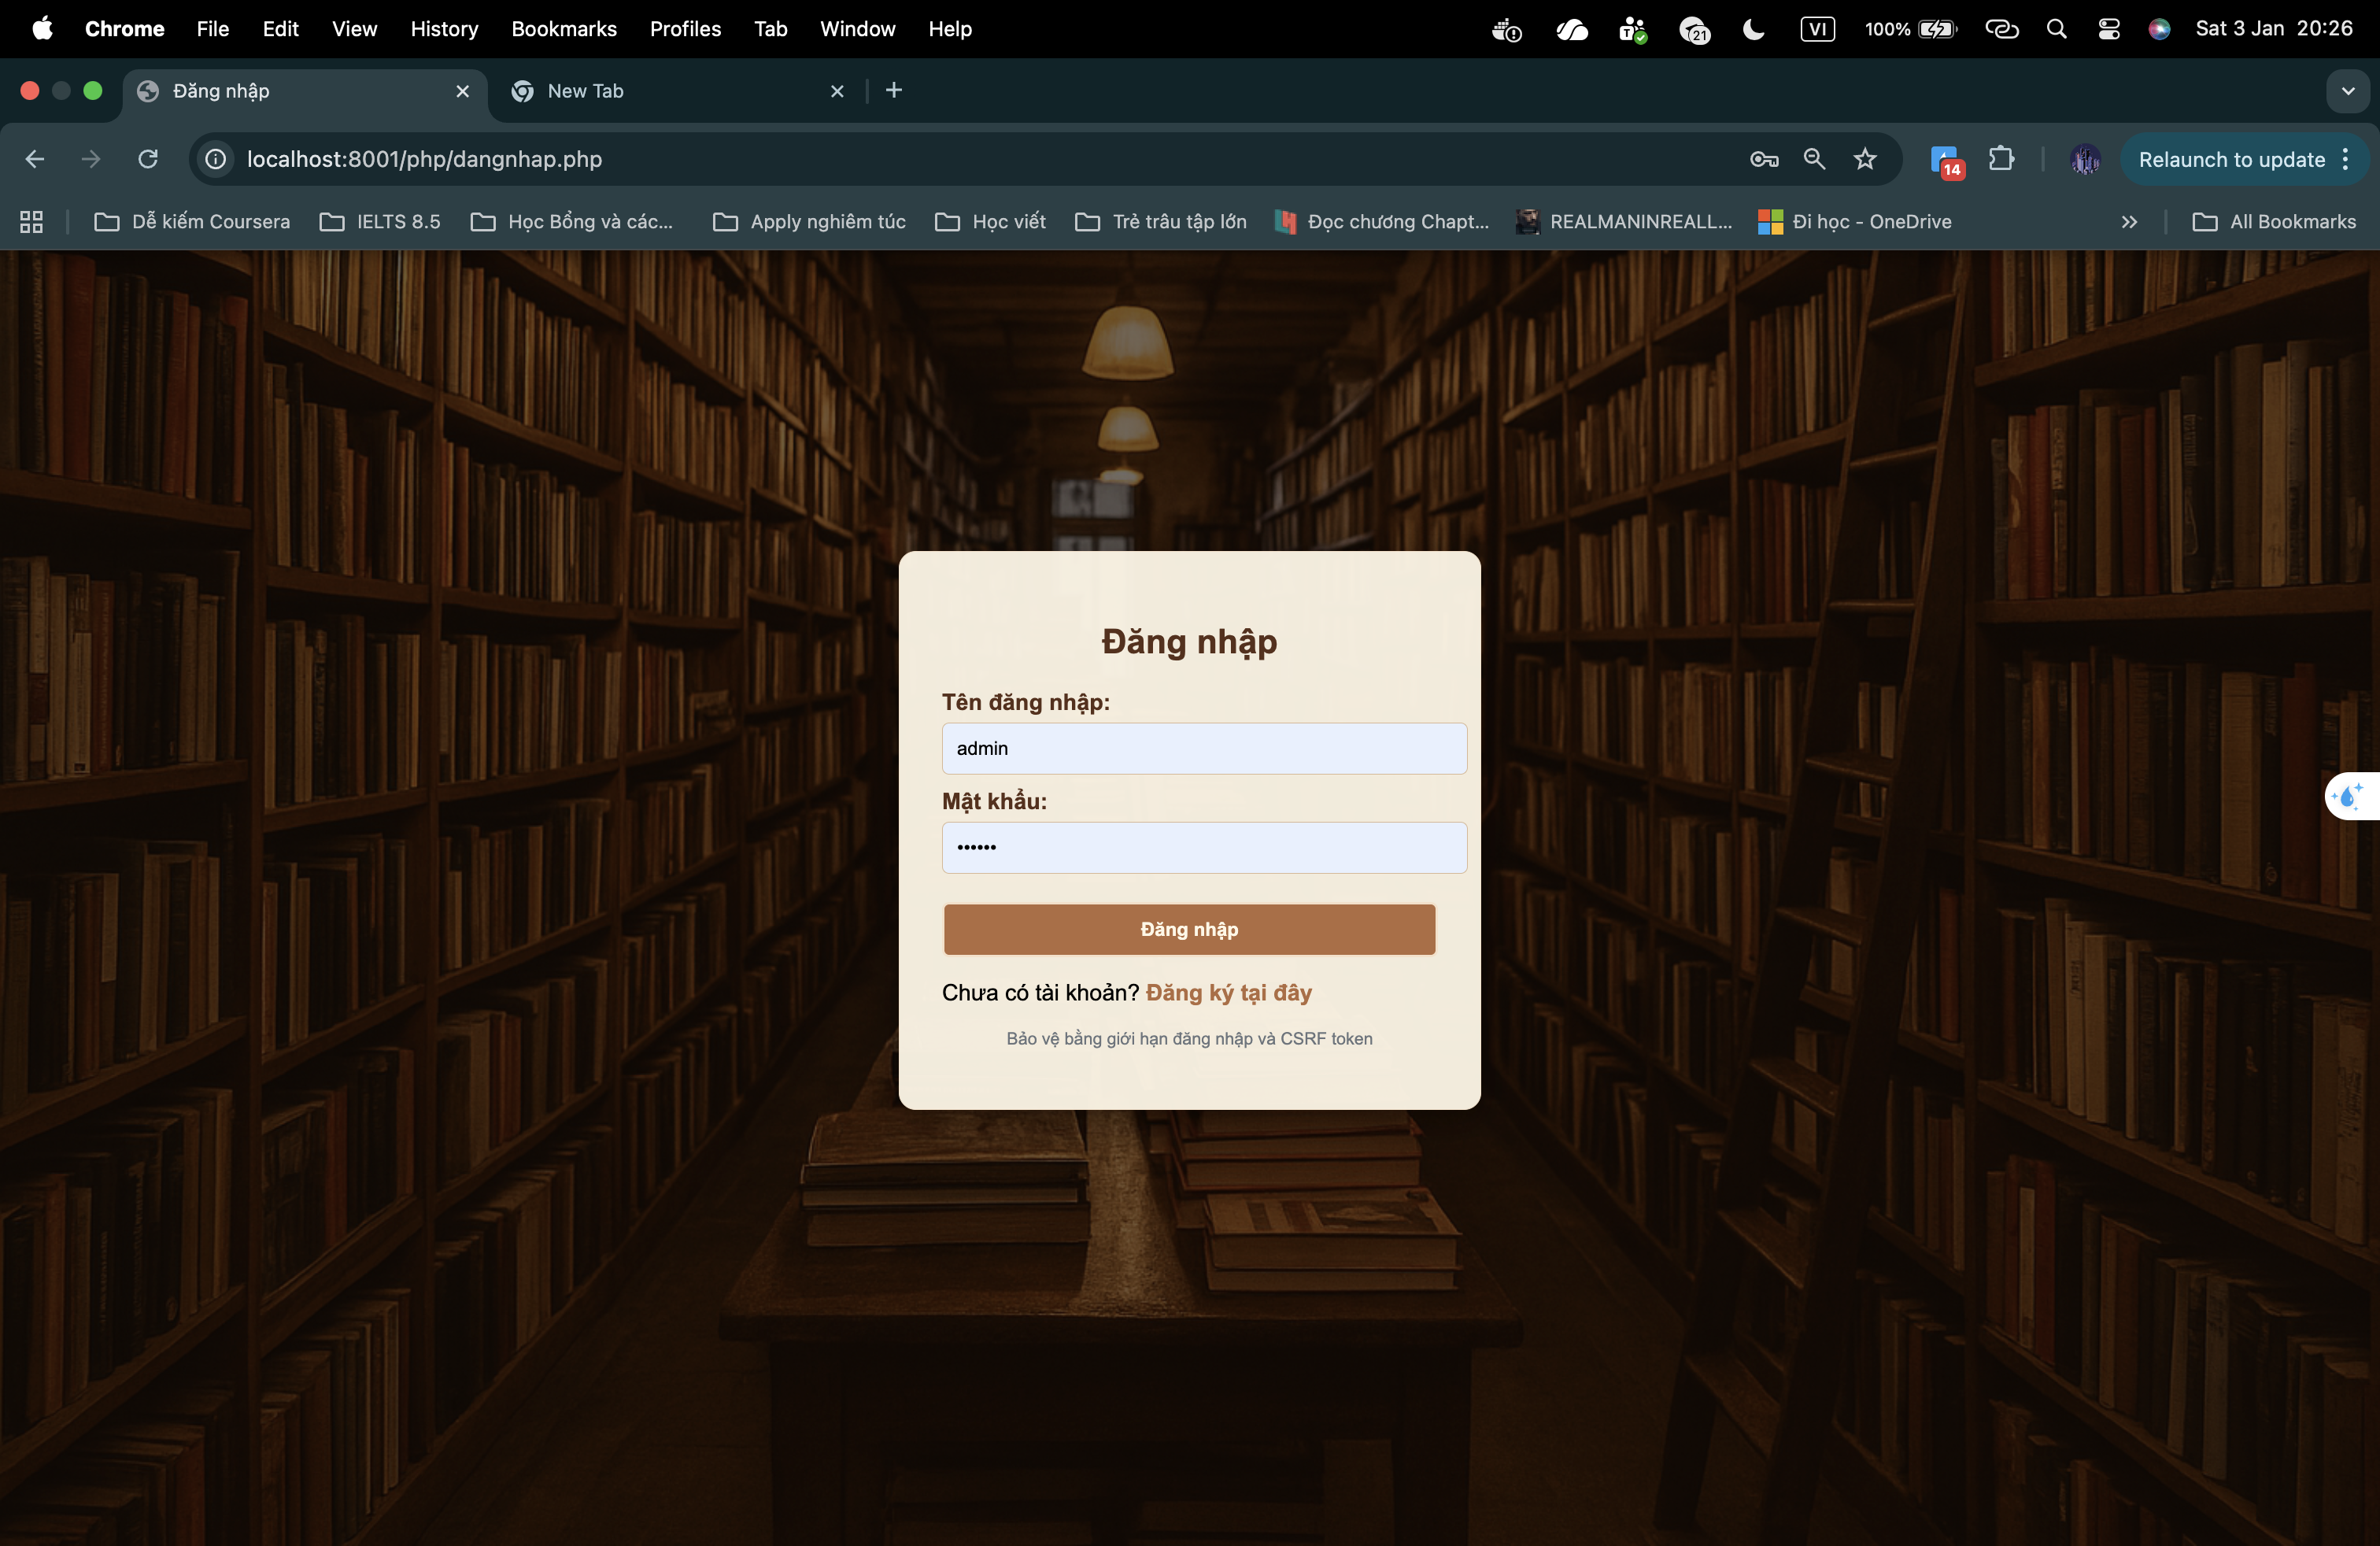
\includegraphics[width=0.85\textwidth]{01_login.png}
    \caption{Giao diện đăng nhập hệ thống}
    \label{fig:login}
\end{figure}

Giao diện đăng nhập hỗ trợ:
\begin{itemize}
    \item Xác thực username/password với bcrypt hash
    \item Phát hiện brute-force attack (lock sau 5 lần thất bại)
    \item Tạo JWT token với thời hạn 24 giờ
    \item Chuyển hướng theo role (admin $\rightarrow$ dashboard, customer $\rightarrow$ danhsachsach)
\end{itemize}

\subsection{Dashboard thống kê (Admin)}

\begin{figure}[H]
    \centering
    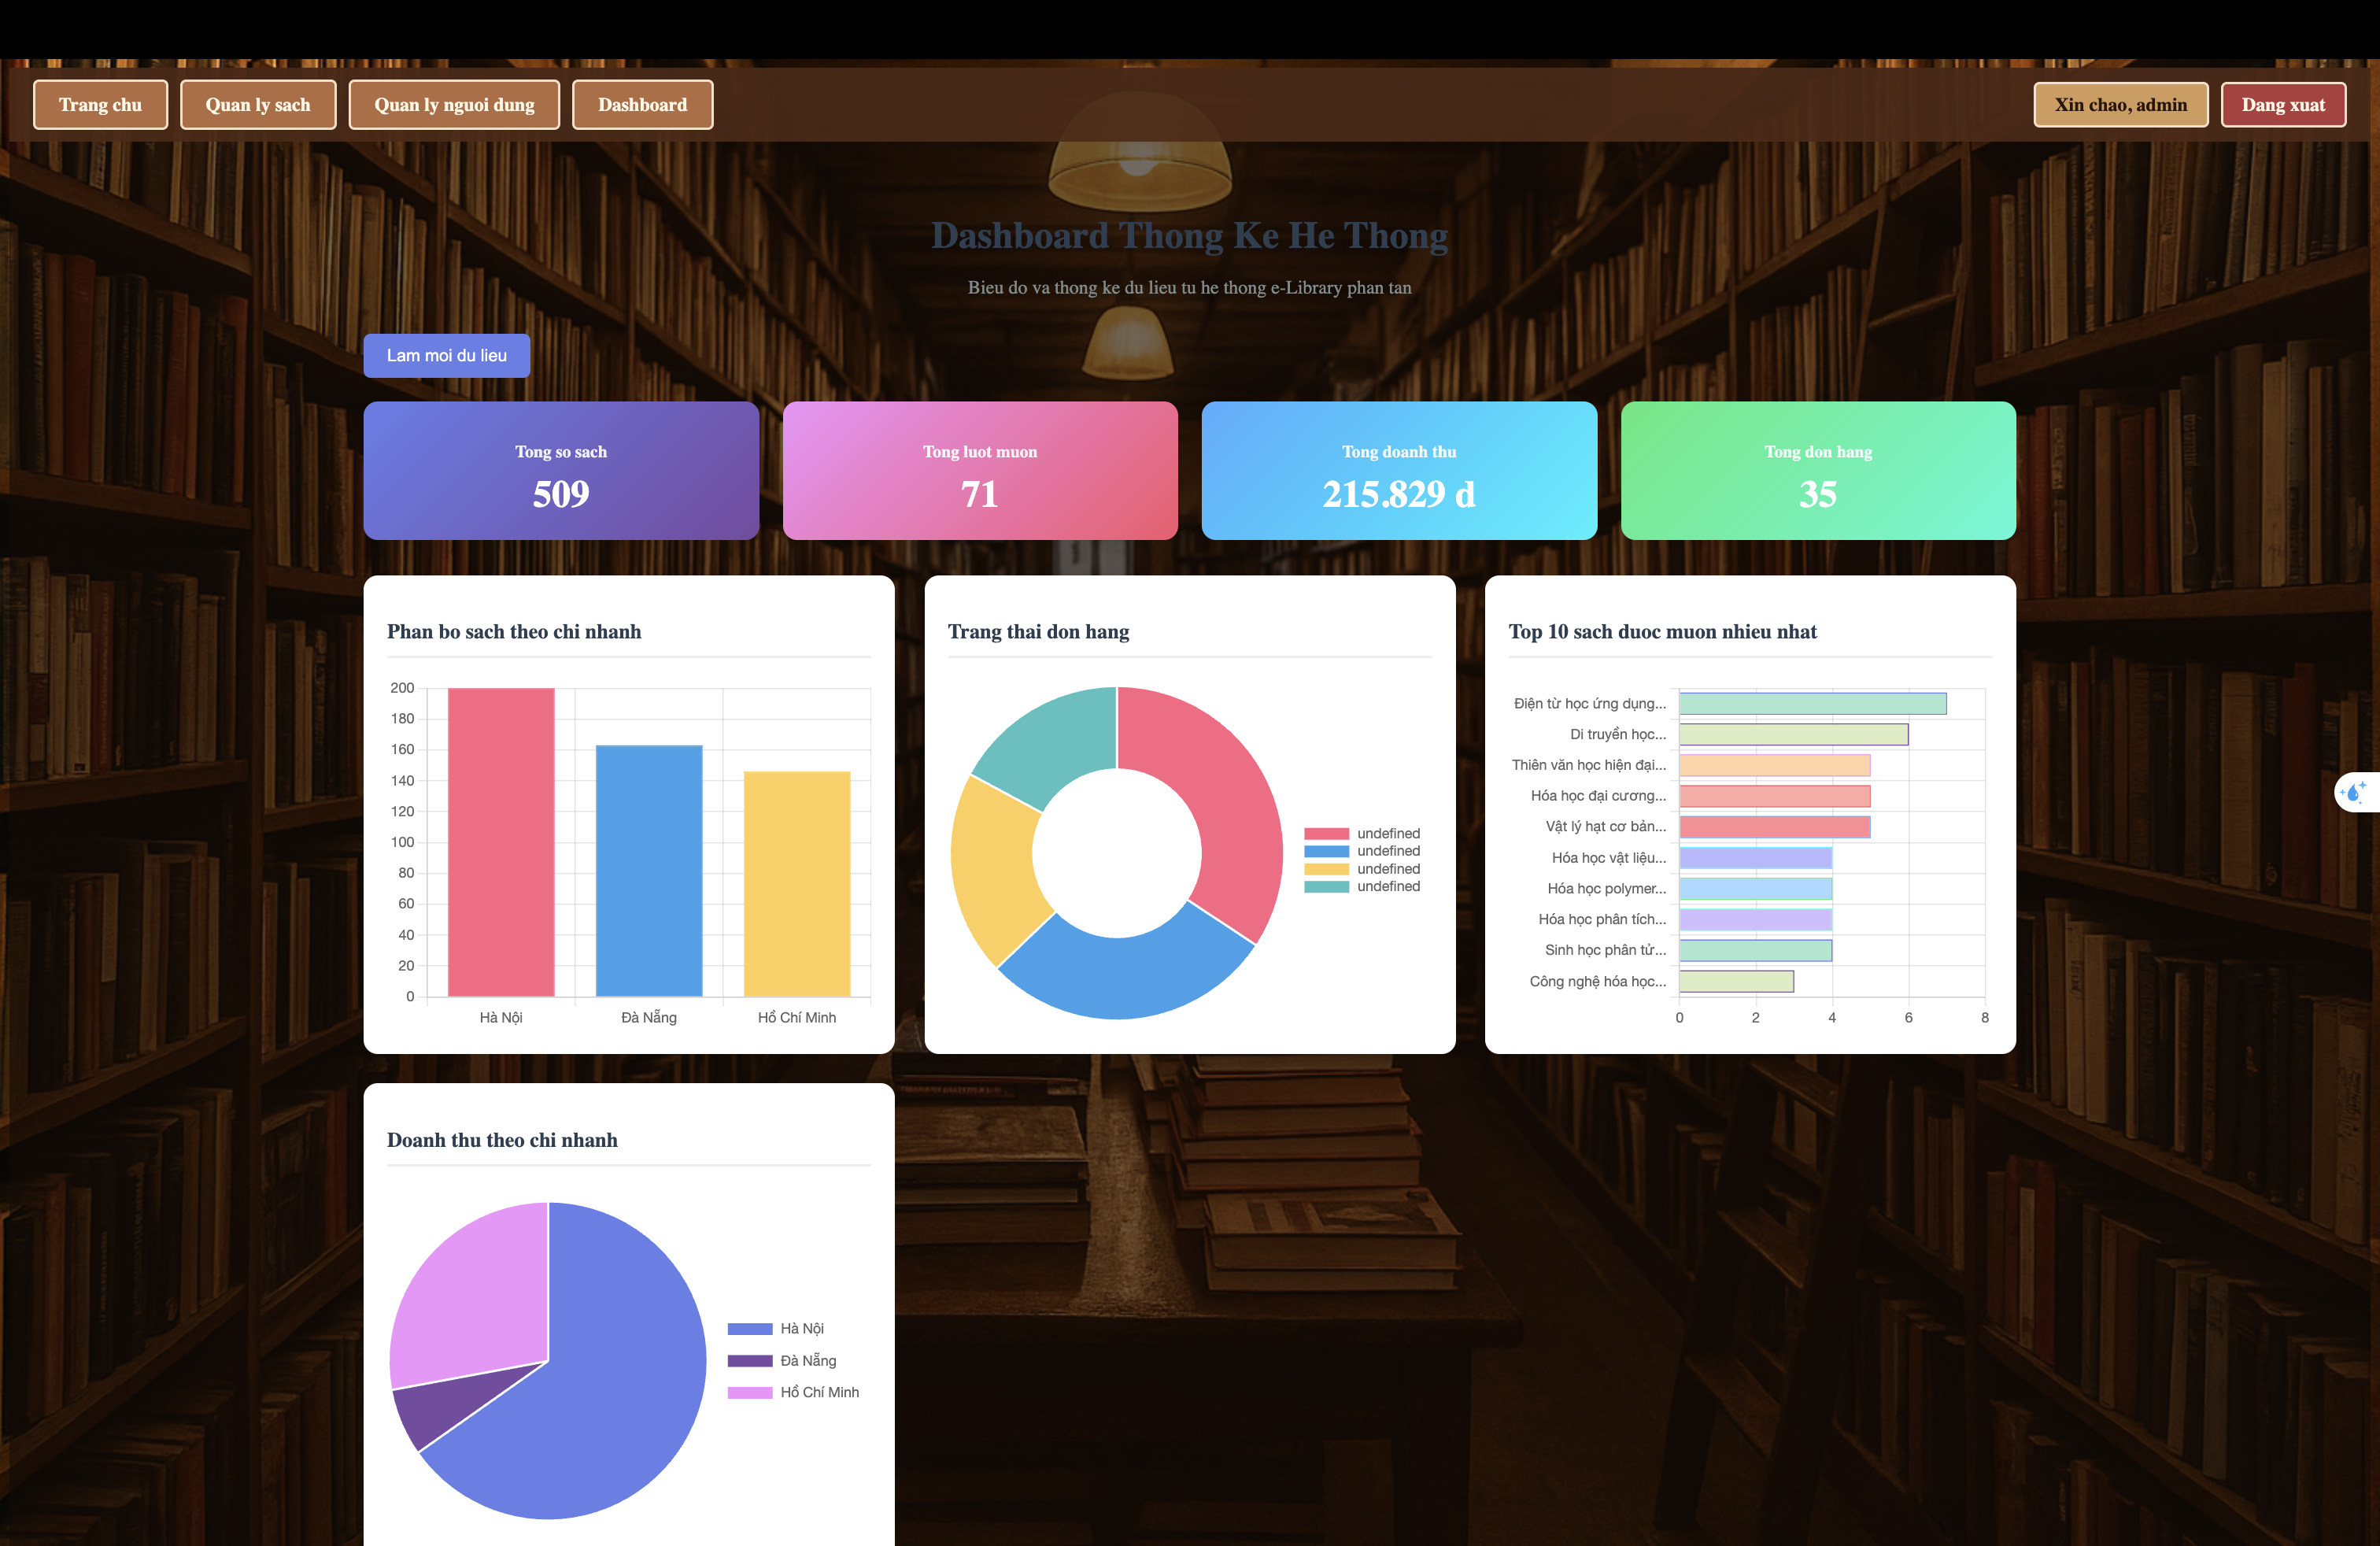
\includegraphics[width=\textwidth]{02_dashboard.png}
    \caption{Dashboard thống kê với biểu đồ Chart.js}
    \label{fig:dashboard}
\end{figure}

Dashboard hiển thị:
\begin{itemize}
    \item Tổng số sách, người dùng, đơn mượn qua cards
    \item Biểu đồ cột: Sách theo chi nhánh
    \item Biểu đồ tròn: Trạng thái đơn hàng
    \item Dữ liệu lấy từ API \texttt{/api/statistics.php}
\end{itemize}

\subsection{Quản lý sách (Admin)}

\begin{figure}[H]
    \centering
    \includegraphics[width=\textwidth]{03_quanlysach.png}
    \caption{Giao diện CRUD quản lý sách}
    \label{fig:quanlysach}
\end{figure}

\subsection{Quản lý người dùng (Admin)}

\begin{figure}[H]
    \centering
    \includegraphics[width=\textwidth]{04_quanlynguoidung.png}
    \caption{Giao diện quản lý người dùng: Danh sách tổng hợp toàn hệ thống}
    \label{fig:quanlynguoidung}
\end{figure}

Giao diện quản lý người dùng hiện tại hiển thị đầy đủ 42 tài khoản, bao gồm 9 quản trị viên tại "Trung Tâm" và 33 khách hàng được đồng bộ từ các chi nhánh (Hà Nội, Đà Nẵng, TP.HCM).

\begin{figure}[H]
    \centering
    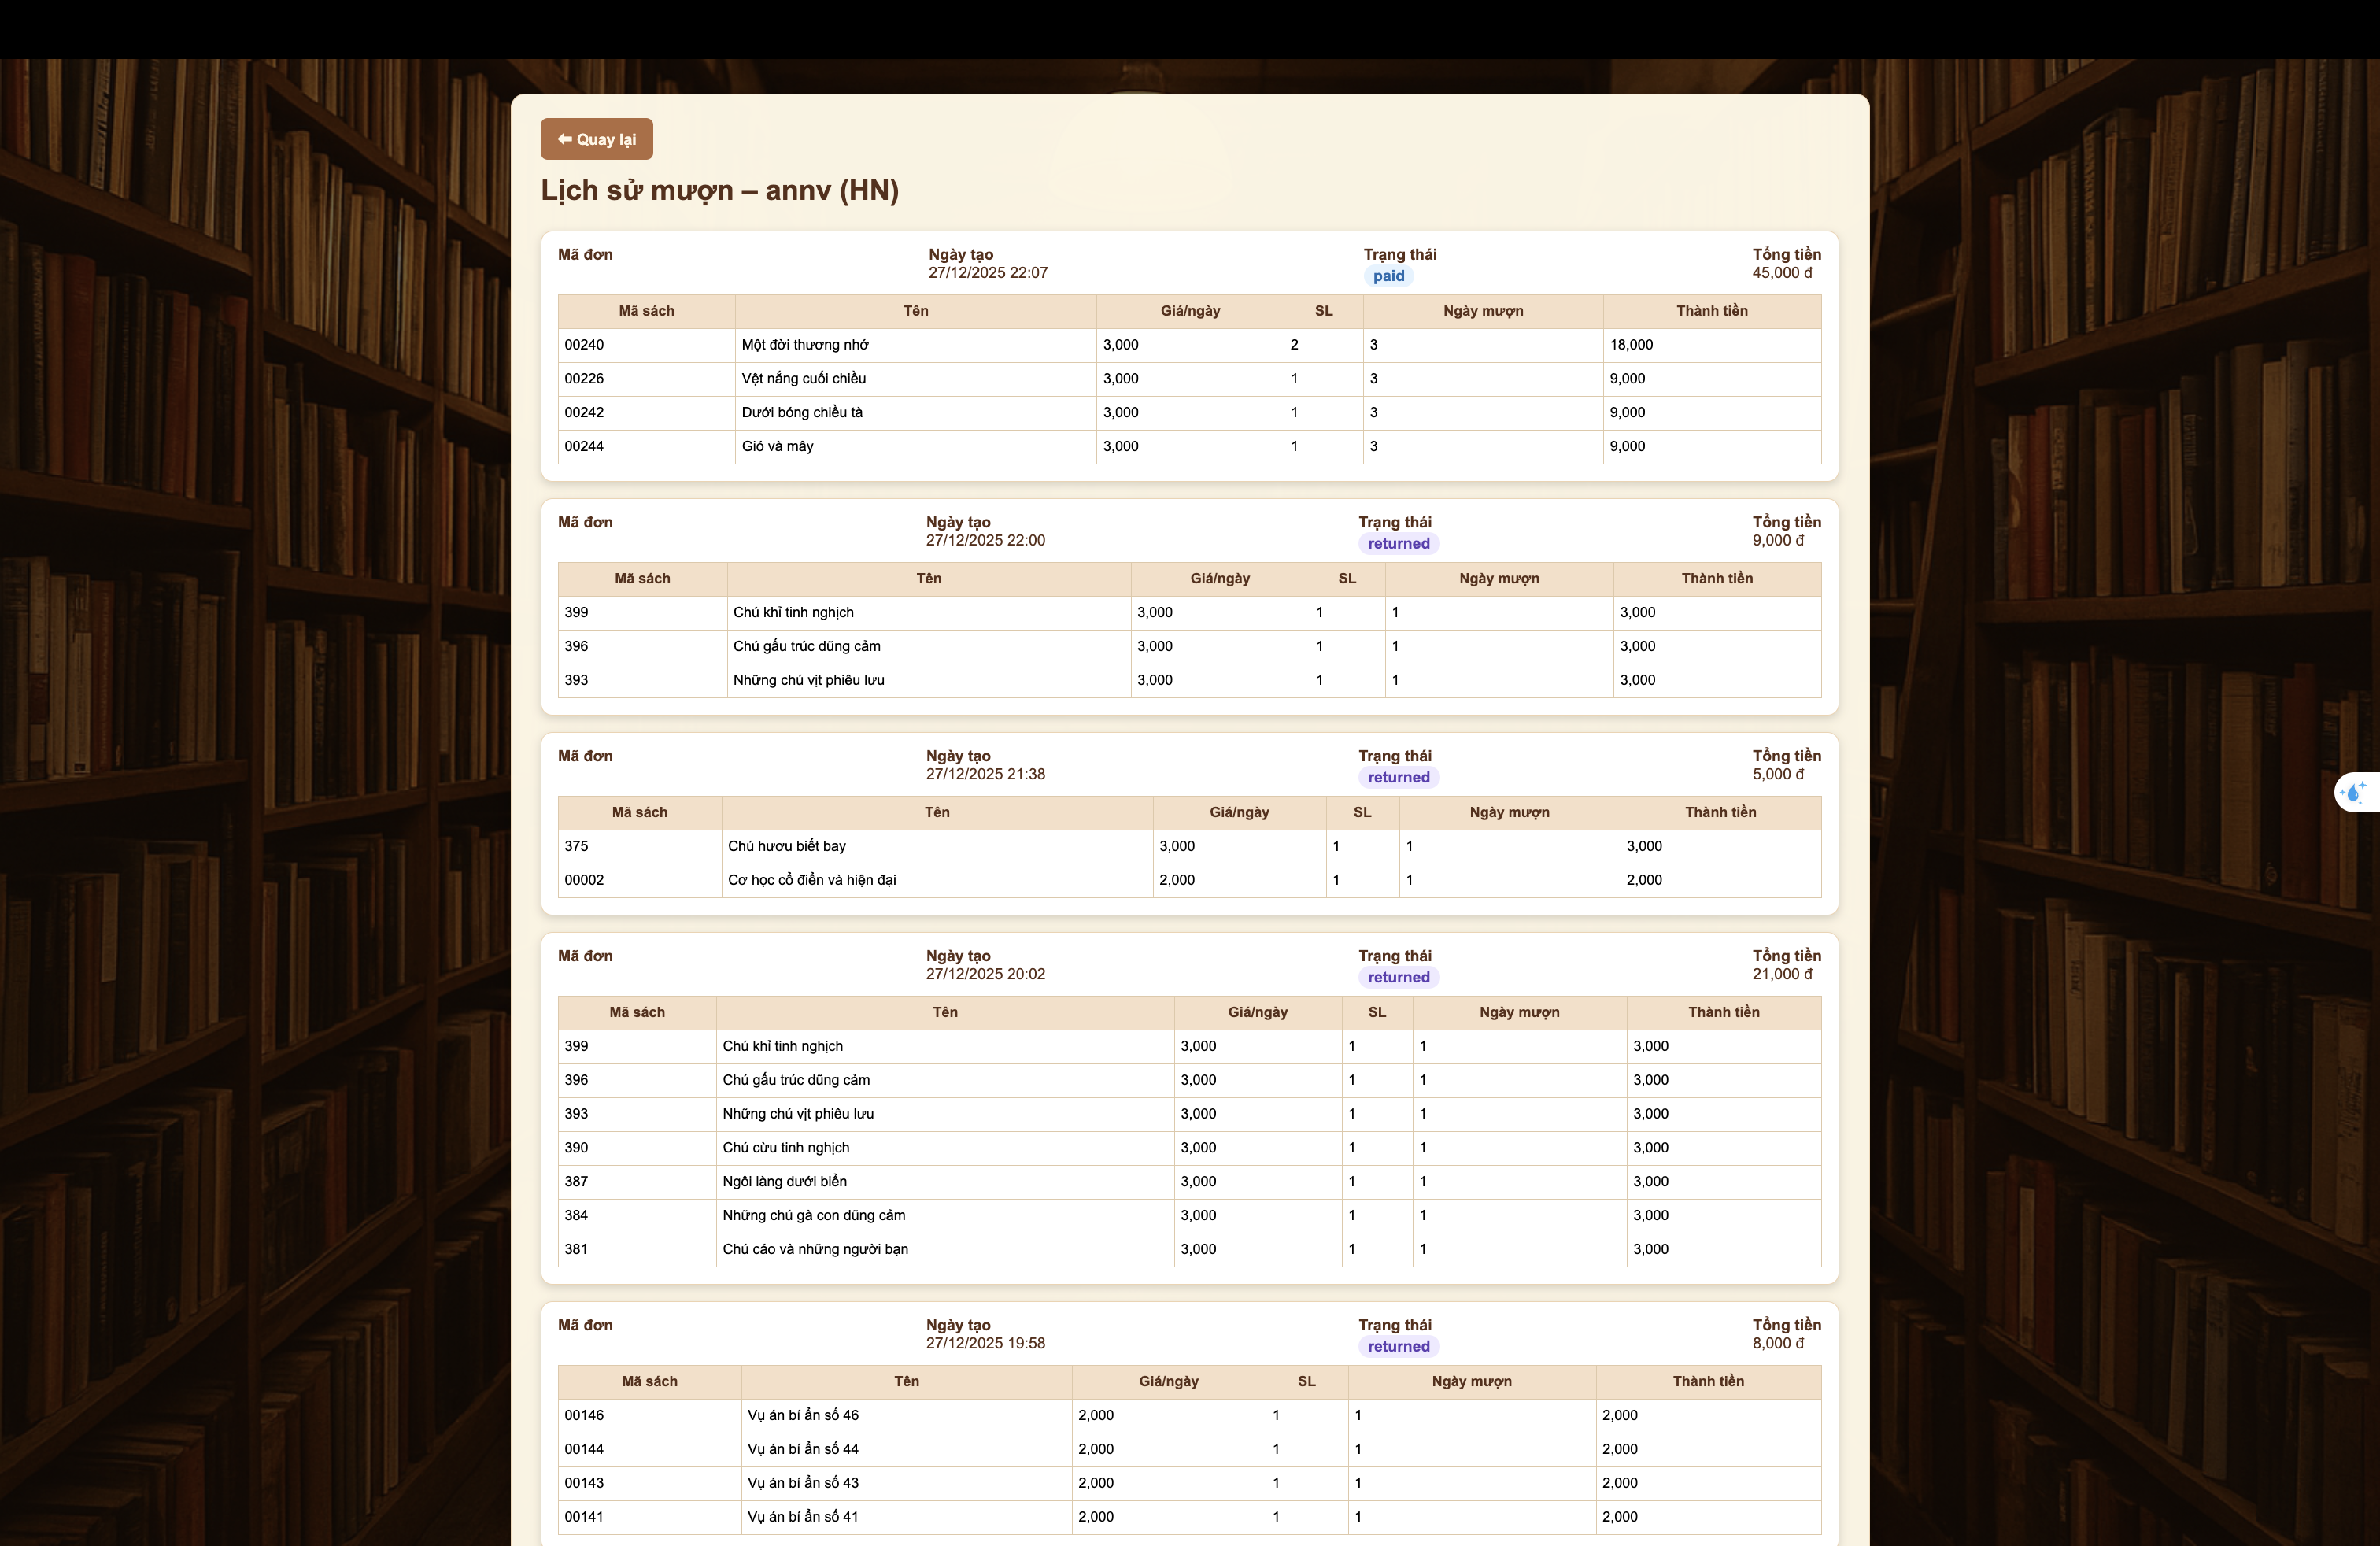
\includegraphics[width=\textwidth]{04_quanlynguoidung_donmuon.png}
    \caption{Chi tiết thống kê đơn mượn: Tổng hợp từ dữ liệu phân tán}
    \label{fig:quanlynguoidung_donmuon}
\end{figure}

Hệ thống tự động tính toán và hiển thị chính xác "Tổng đơn mượn" cho từng người dùng bằng cách cộng gộp dữ liệu từ cơ sở dữ liệu trung tâm và các đơn hàng được đồng bộ từ chi nhánh, đảm bảo tính nhất quán của báo cáo.


\subsection{Danh sách sách (Customer)}

\begin{figure}[H]
    \centering
    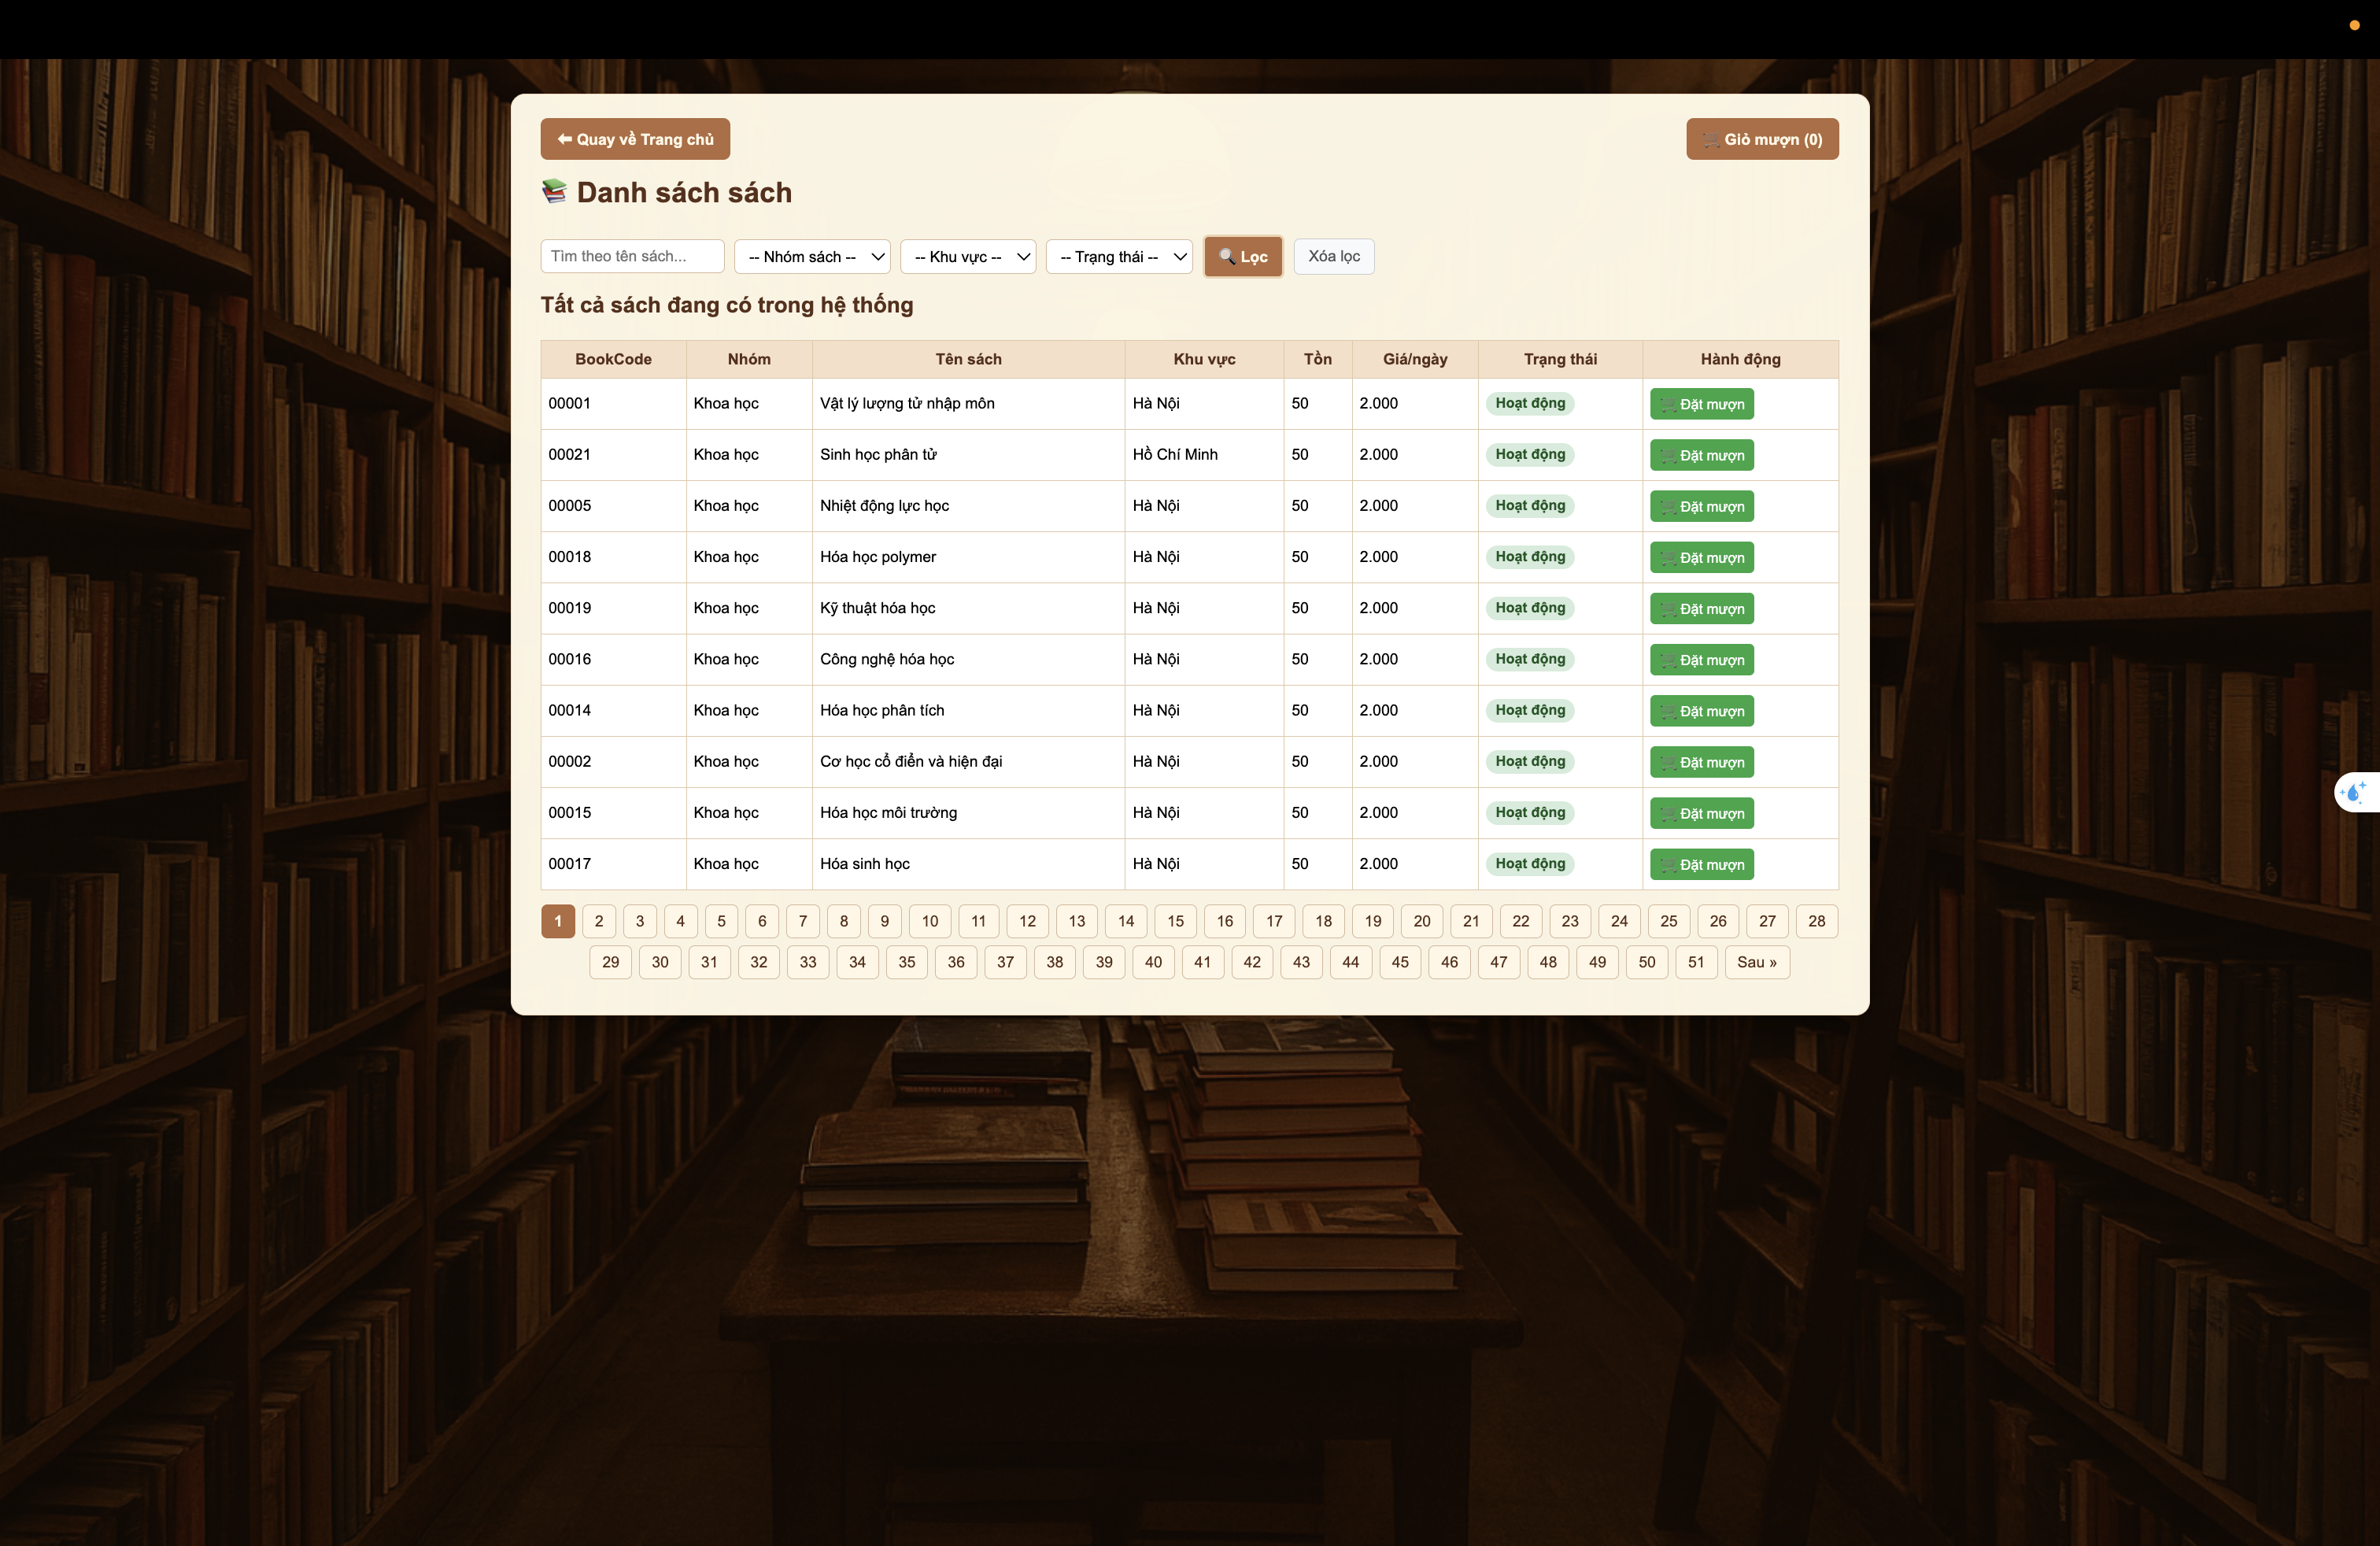
\includegraphics[width=\textwidth]{05_danhsachsach.png}
    \caption{Danh sách sách cho khách hàng}
    \label{fig:danhsachsach}
\end{figure}

\subsection{Giỏ hàng mượn sách}

\begin{figure}[H]
    \centering
    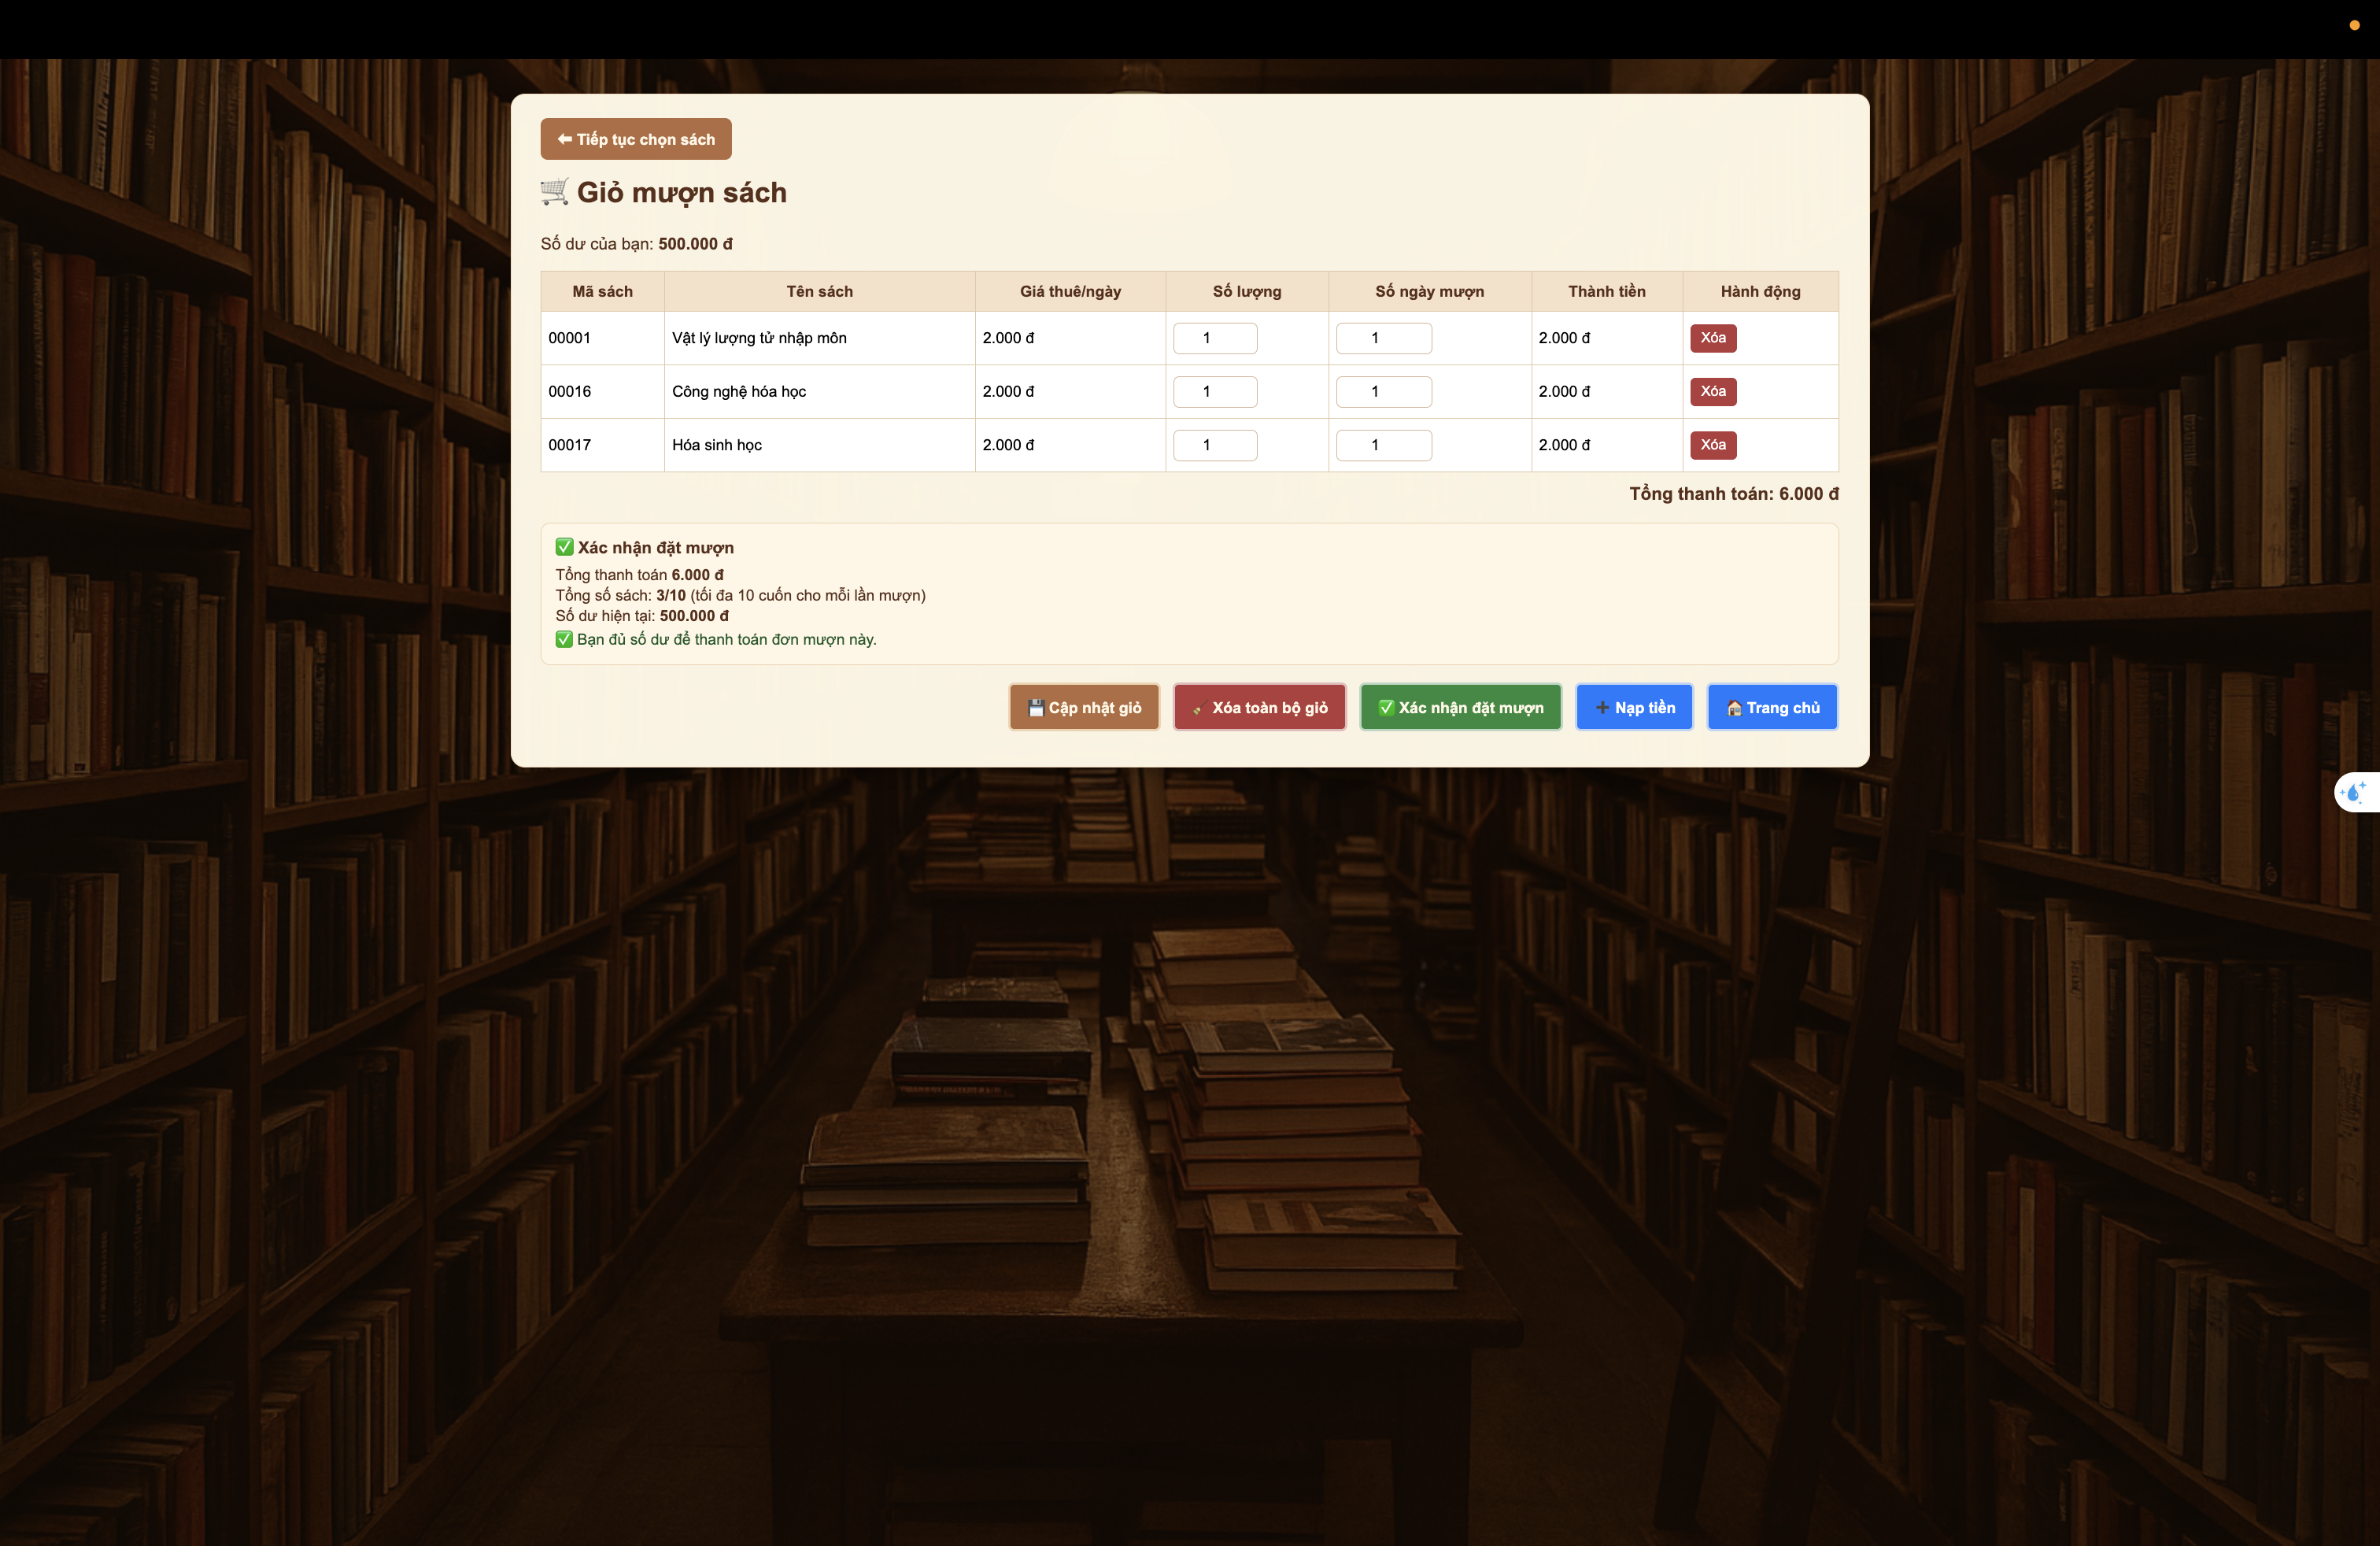
\includegraphics[width=\textwidth]{06_giohang.png}
    \caption{Giao diện giỏ hàng mượn sách}
    \label{fig:giohang}
\end{figure}

\subsection{Dữ liệu Chi nhánh (Mô hình Phân tán)}

\begin{figure}[H]
    \centering
    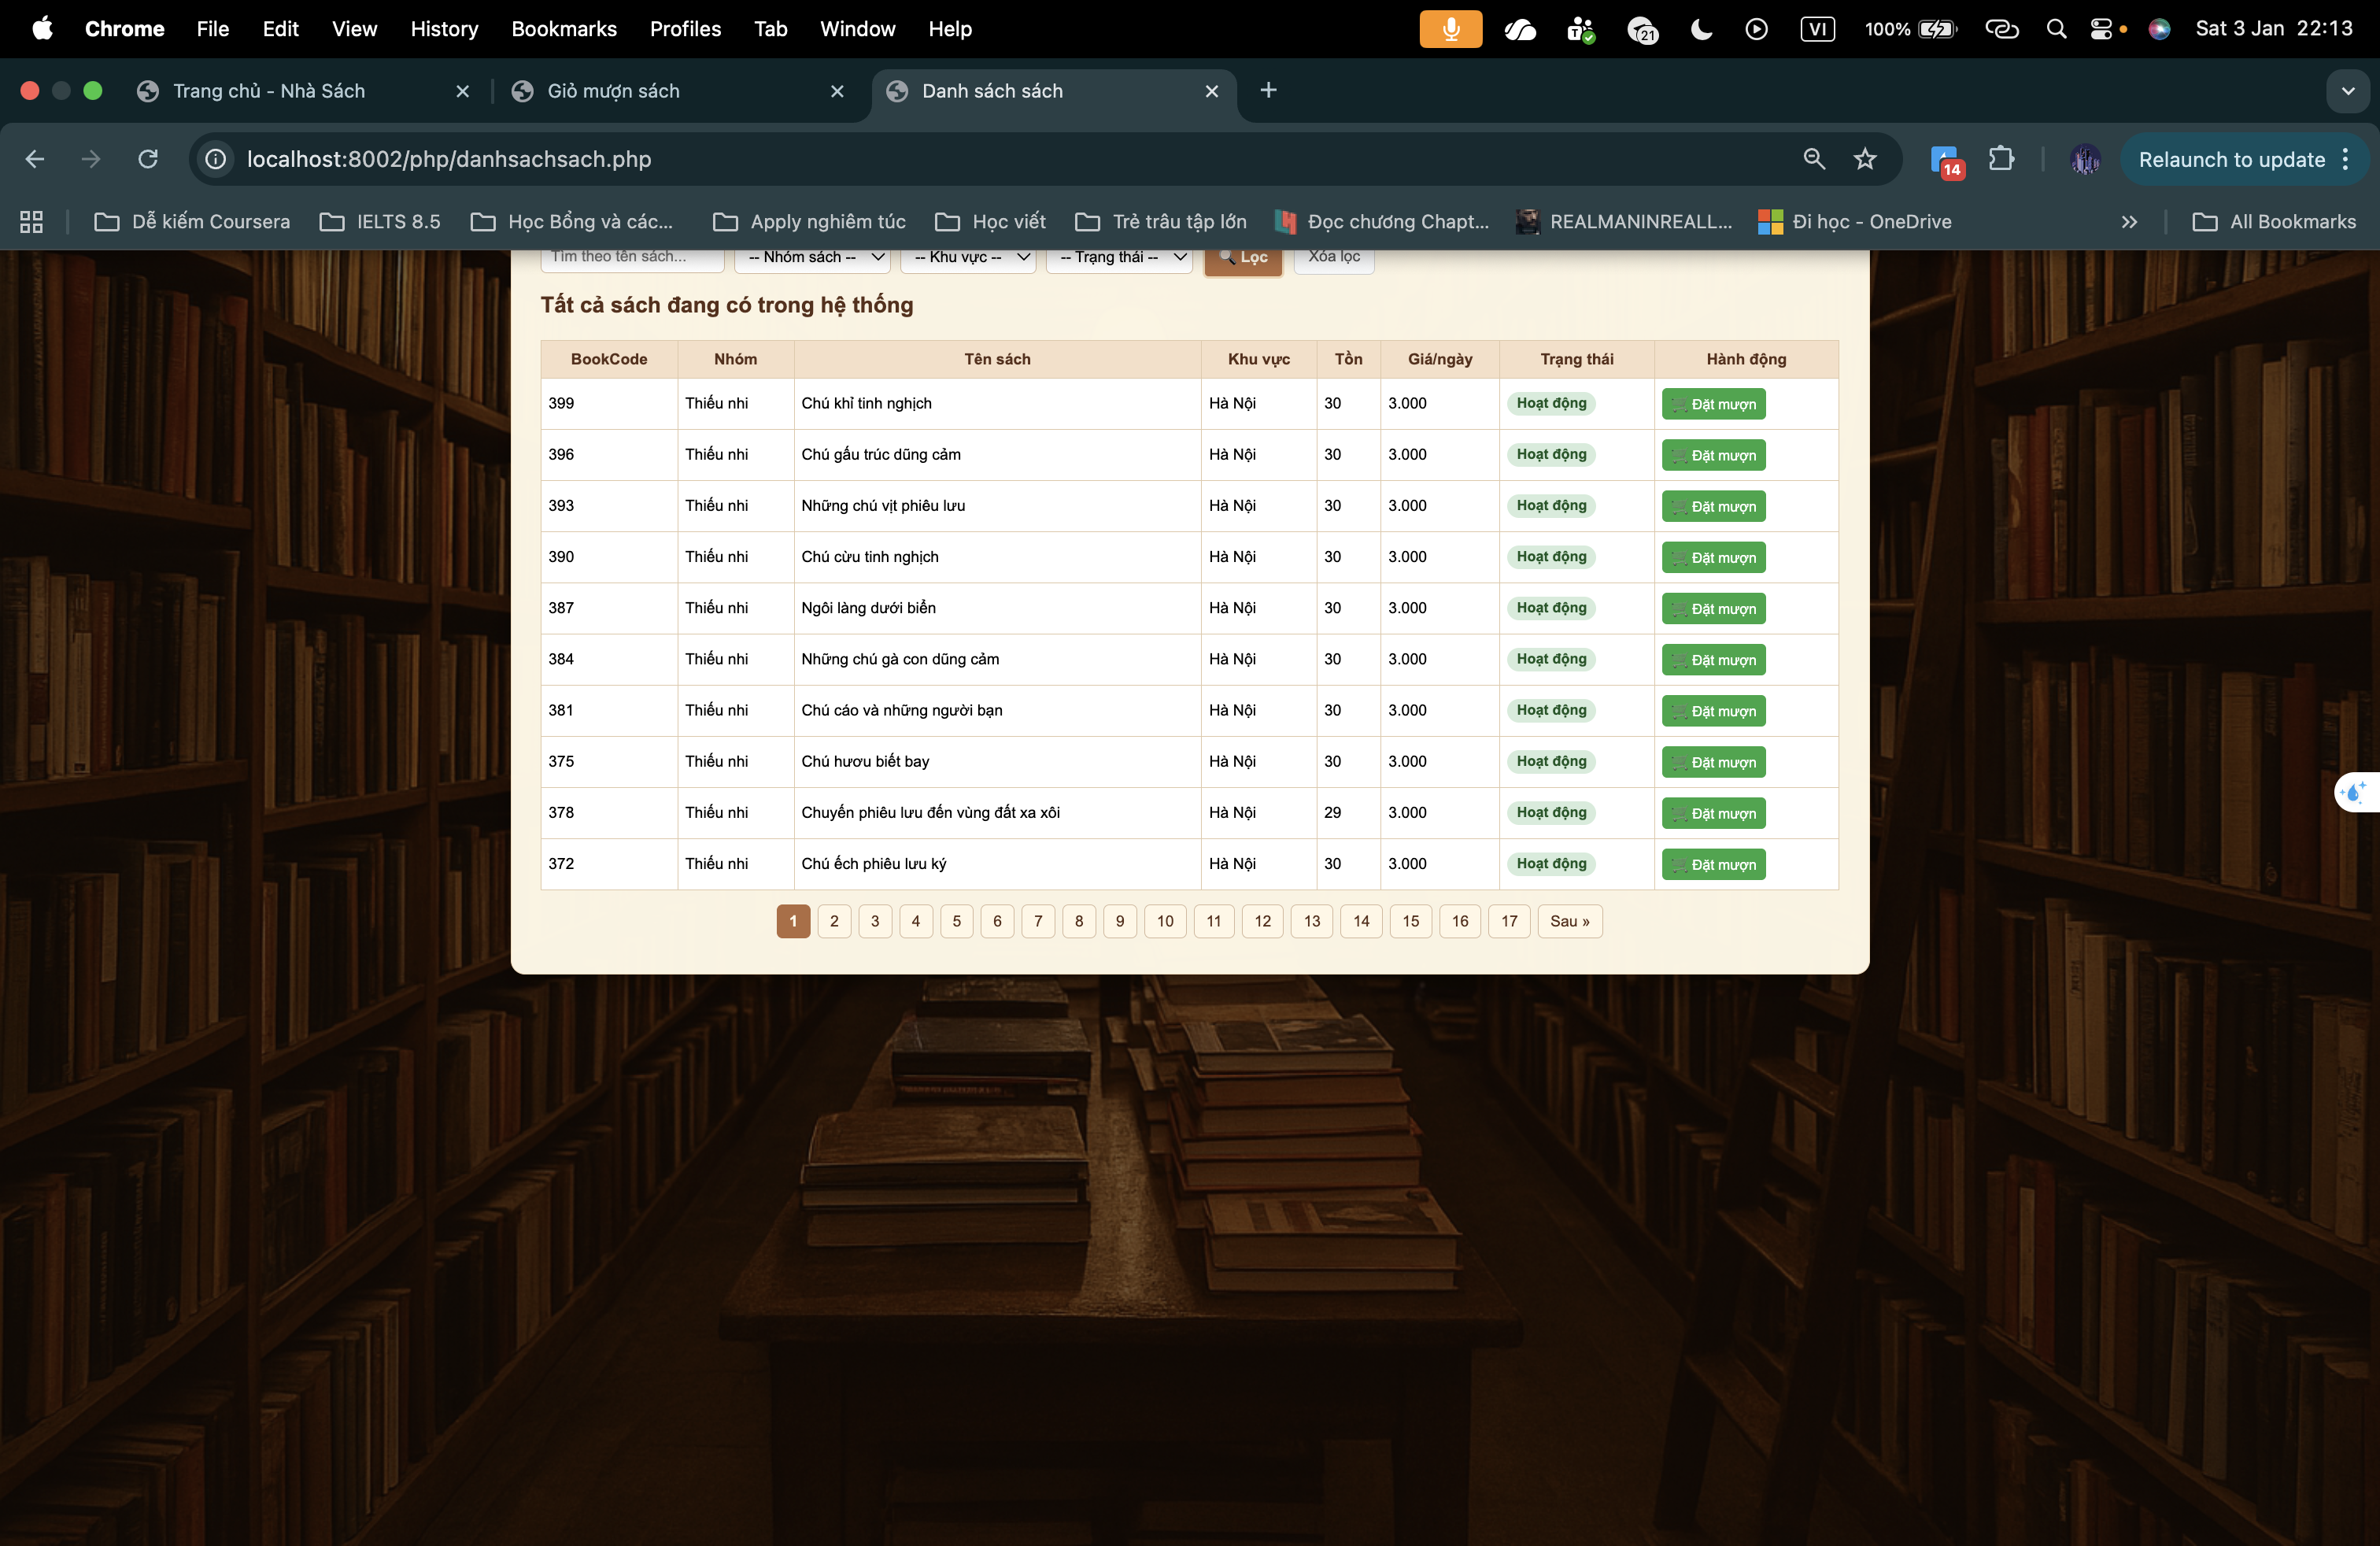
\includegraphics[width=\textwidth]{07_branch_books.png}
    \caption{Danh sách sách tại chi nhánh Hà Nội}
    \label{fig:branch_books}
\end{figure}

\begin{figure}[H]
    \centering
    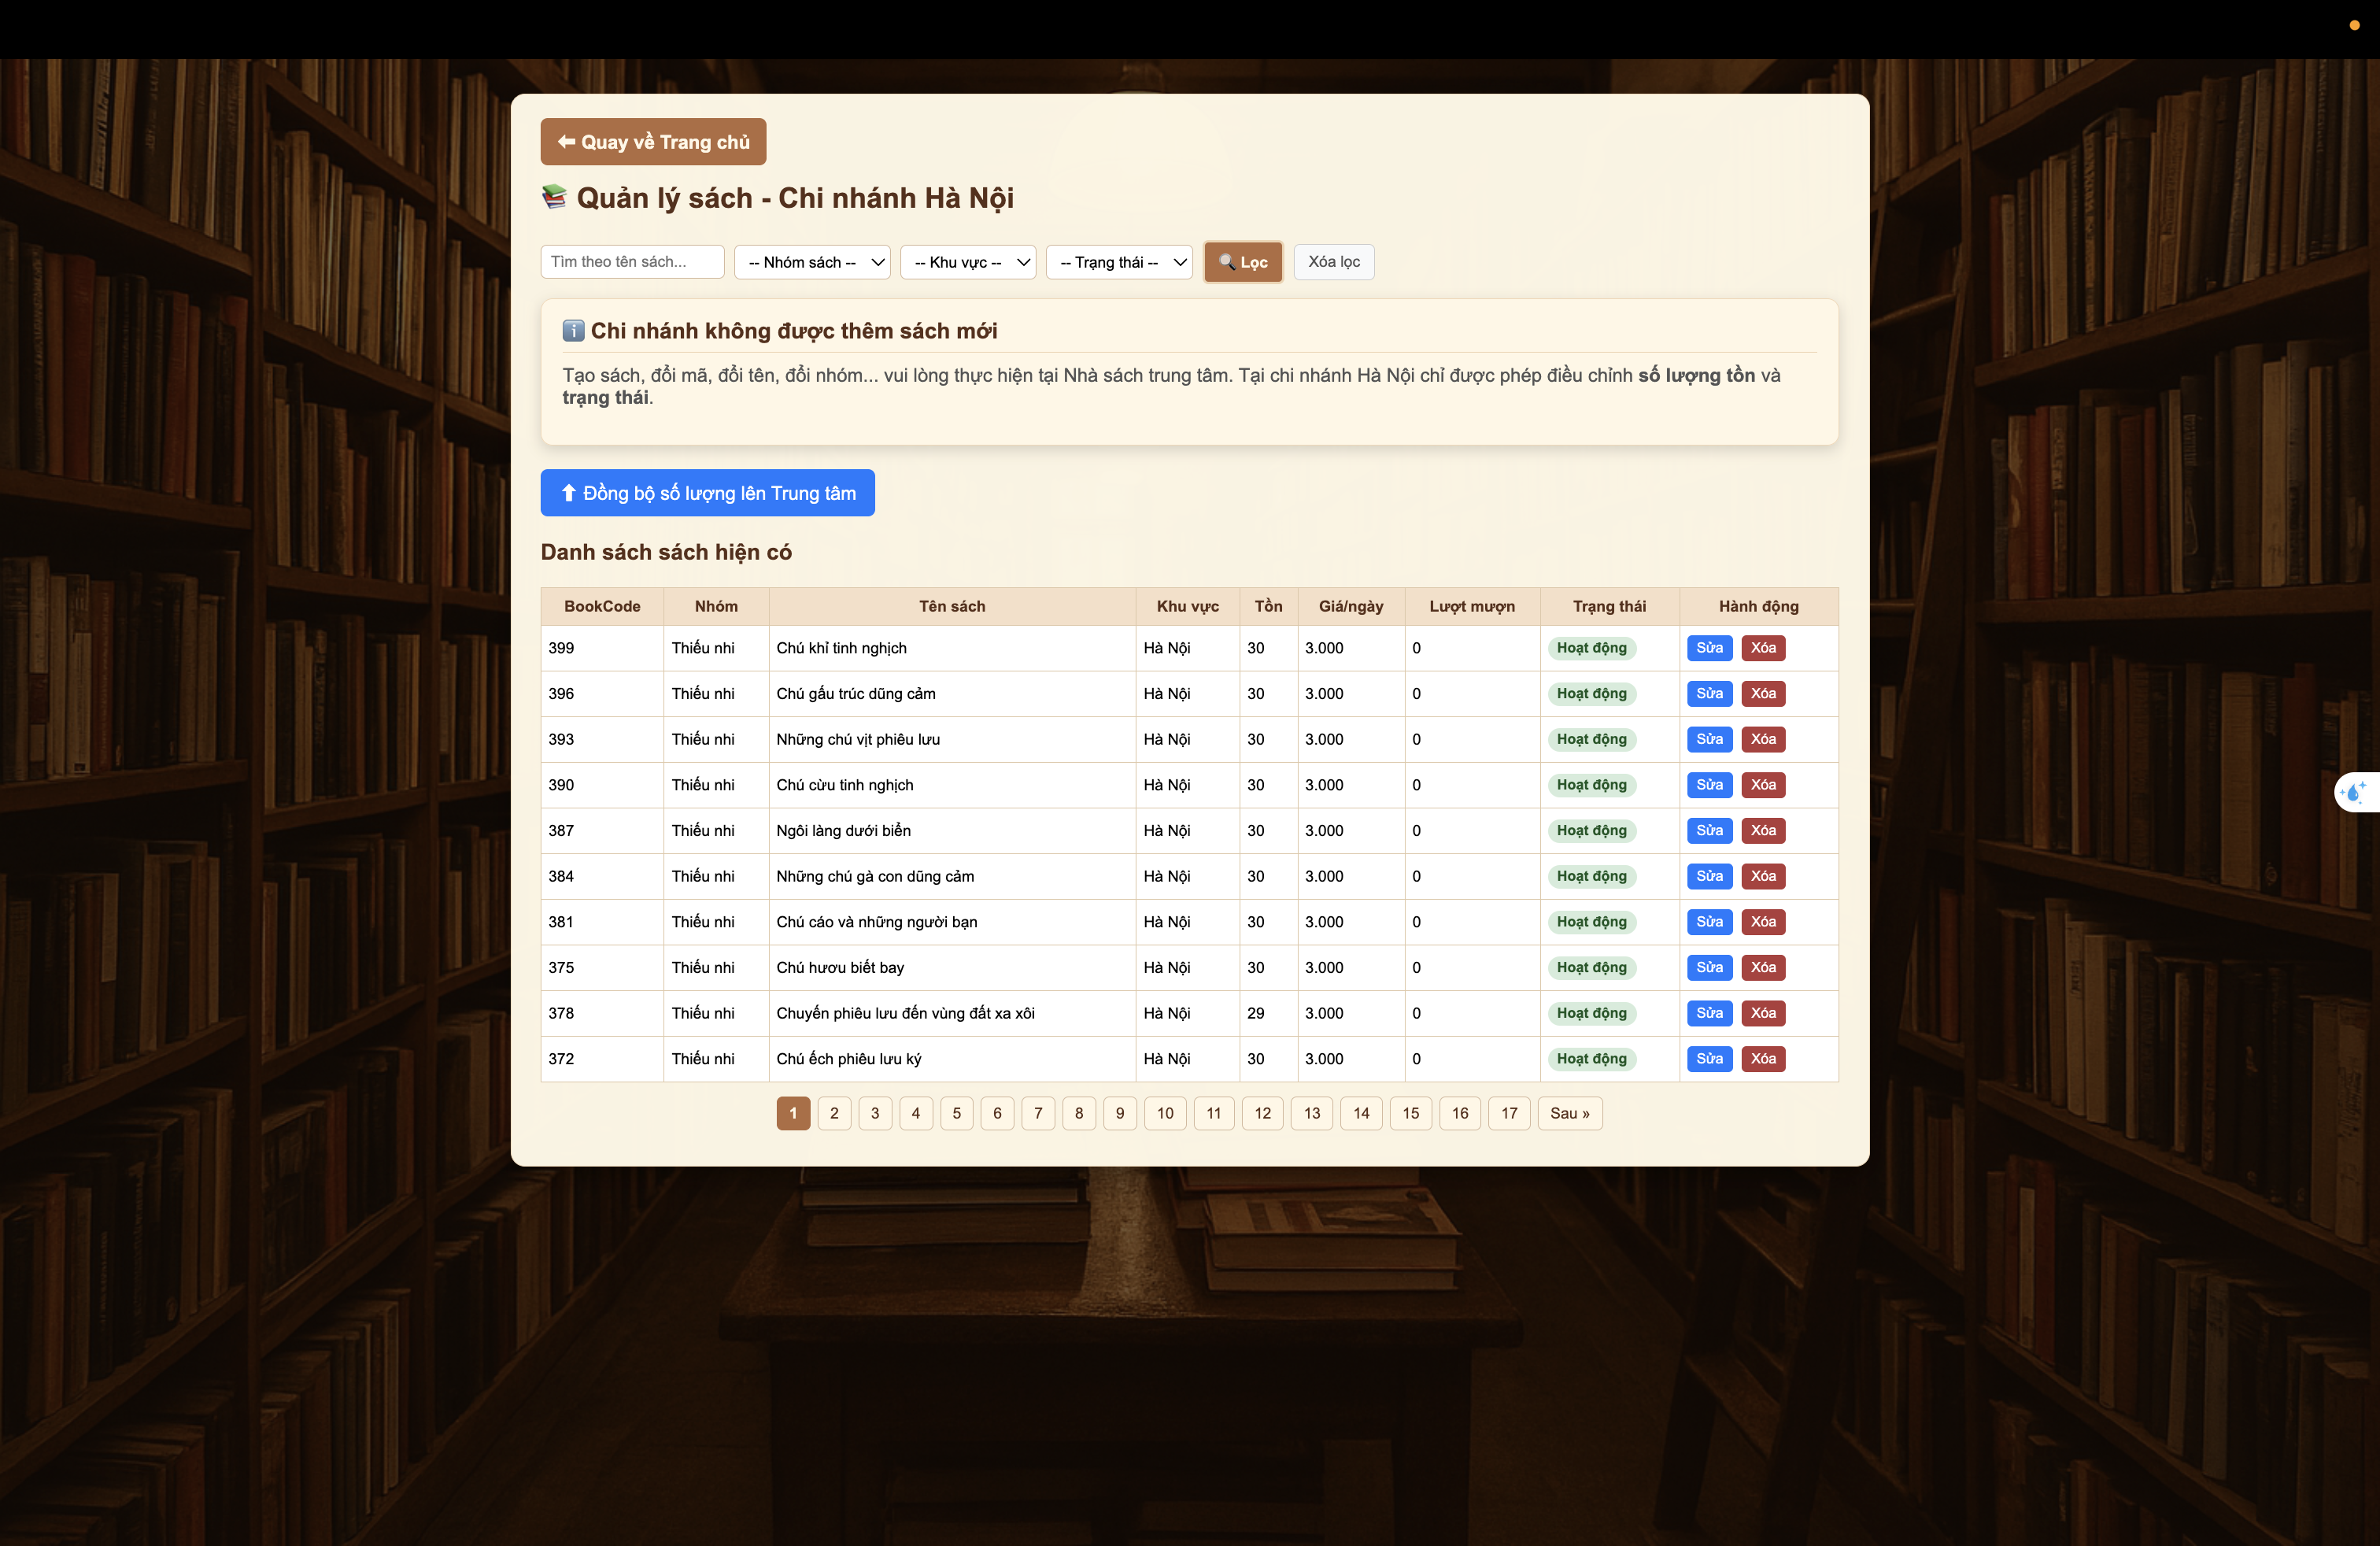
\includegraphics[width=\textwidth]{09_branch_admin.png}
    \caption{Giao diện Admin quản lý tại chi nhánh}
    \label{fig:branch_admin}
\end{figure}

\subsection{Docker Containers}

\begin{figure}[H]
    \centering
    \includegraphics[width=0.8\textwidth]{10_docker.png}
    \caption{Docker Desktop hiển thị MongoDB containers}
    \label{fig:docker}
\end{figure}

\subsection{MongoDB Compass}

\begin{figure}[H]
    \centering
    \includegraphics[width=\textwidth]{11_mongodb_compass.png}
    \caption{MongoDB Compass hiển thị collection books}
    \label{fig:compass}
\end{figure}

\section{Triển khai Aggregation Pipeline}

\subsection{Tổng quan API Statistics}

Hệ thống cung cấp 8 endpoints thống kê sử dụng Aggregation Pipeline trong file \texttt{api/statistics.php}:

\begin{table}[H]
\centering
\caption{Danh sách Aggregation Pipeline endpoints}
\begin{tabular}{|c|l|l|}
\hline
\textbf{\#} & \textbf{Action} & \textbf{Pipeline Stages} \\
\hline
1 & books\_by\_location & \$match, \$group, \$sort, \$project \\
2 & popular\_books & \$match, \$sort, \$limit, \$project \\
3 & revenue\_by\_date & \$match, \$addFields, \$group, \$sort, \$project \\
4 & user\_statistics & \$match, \$group, \$sort, \$limit, \$addFields, \$project \\
5 & user\_details & \$match, \textbf{\$lookup}, \$unwind, \$group, \$sort, \$limit \\
6 & order\_status\_summary & \$group, \$sort, \$project \\
7 & monthly\_trends & \$match, \$addFields, \$group, \$sort, \$project \\
8 & book\_group\_stats & \$match, \textbf{\$facet}, \textbf{\$bucket} \\
\hline
\end{tabular}
\end{table}

\subsection{Endpoint books\_by\_location}

\begin{lstlisting}[language=PHP, caption=statistics.php - books\_by\_location với 4 stages]
case 'books_by_location':
    $pipeline = [
        // Stage 1: $match - Filter active books
        ['$match' => ['status' => ['$ne' => 'deleted']]],

        // Stage 2: $group - Aggregate by location
        ['$group' => [
            '_id' => '$location',
            'totalBooks' => ['$sum' => 1],
            'totalQuantity' => ['$sum' => '$quantity'],
            'avgPricePerDay' => ['$avg' => '$pricePerDay'],
            'totalBorrowCount' => ['$sum' => '$borrowCount']
        ]],

        // Stage 3: $sort - Order by total books
        ['$sort' => ['totalBooks' => -1]],

        // Stage 4: $project - Rename and format fields
        ['$project' => [
            '_id' => 0,
            'location' => '$_id',
            'totalBooks' => 1,
            'totalQuantity' => 1,
            'avgPricePerDay' => ['$round' => ['$avgPricePerDay', 0]],
            'totalBorrowCount' => 1
        ]]
    ];

    $result = $db->books->aggregate($pipeline)->toArray();
\end{lstlisting}

\subsection{Endpoint user\_details với \$lookup JOIN}

Đây là endpoint quan trọng nhất, thể hiện khả năng JOIN giữa các collections trong MongoDB:

\begin{lstlisting}[language=PHP, caption=statistics.php - user\_details với \$lookup]
case 'user_details':
    $pipeline = [
        // Stage 1: Match completed orders
        ['$match' => ['status' => ['$in' => ['paid', 'success', 'returned']]]],

        // Stage 2: $lookup - LEFT OUTER JOIN with users collection
        ['$lookup' => [
            'from' => 'users',           // Target collection
            'localField' => 'user_id',   // Field in orders
            'foreignField' => '_id',     // Field in users
            'as' => 'user_info'          // Output array
        ]],

        // Stage 3: $unwind - Flatten user_info array
        ['$unwind' => [
            'path' => '$user_info',
            'preserveNullAndEmptyArrays' => true
        ]],

        // Stage 4: Group by user with joined info
        ['$group' => [
            '_id' => '$user_id',
            'username' => ['$first' => '$username'],
            'email' => ['$first' => '$user_info.email'],
            'fullname' => ['$first' => '$user_info.fullname'],
            'role' => ['$first' => '$user_info.role'],
            'totalOrders' => ['$sum' => 1],
            'totalSpent' => ['$sum' => '$total_amount']
        ]],

        ['$sort' => ['totalSpent' => -1]],
        ['$limit' => 20]
    ];

    $result = $db->orders->aggregate($pipeline)->toArray();
\end{lstlisting}

\subsection{Endpoint book\_group\_stats với \$facet và \$bucket}

\begin{lstlisting}[language=PHP, caption=statistics.php - Multi-faceted statistics]
case 'book_group_stats':
    $pipeline = [
        ['$match' => ['status' => ['$ne' => 'deleted']]],

        ['$facet' => [
            // Facet 1: Statistics by book group
            'byGroup' => [
                ['$group' => [
                    '_id' => '$bookGroup',
                    'count' => ['$sum' => 1],
                    'totalQuantity' => ['$sum' => '$quantity']
                ]],
                ['$sort' => ['count' => -1]]
            ],

            // Facet 2: Overall summary
            'summary' => [
                ['$group' => [
                    '_id' => null,
                    'totalBooks' => ['$sum' => 1],
                    'avgPrice' => ['$avg' => '$pricePerDay'],
                    'totalBorrows' => ['$sum' => '$borrowCount']
                ]]
            ],

            // Facet 3: Price distribution with $bucket
            'priceRanges' => [
                ['$bucket' => [
                    'groupBy' => '$pricePerDay',
                    'boundaries' => [0, 5000, 10000, 20000, 50000, 100000],
                    'default' => 'Other',
                    'output' => ['count' => ['$sum' => 1]]
                ]]
            ]
        ]]
    ];
\end{lstlisting}

\section{Triển khai Map-Reduce}

\subsection{Tổng quan API Map-Reduce}

File \texttt{api/mapreduce.php} cung cấp 5 Map-Reduce operations:

\begin{table}[H]
\centering
\caption{Danh sách Map-Reduce operations}
\begin{tabular}{|c|l|l|}
\hline
\textbf{\#} & \textbf{Action} & \textbf{Mô tả} \\
\hline
1 & borrow\_stats & Thống kê mượn sách theo bookCode \\
2 & revenue\_by\_user & Doanh thu theo user \\
3 & books\_by\_category & Sách theo thể loại \\
4 & daily\_activity & Hoạt động theo ngày \\
5 & location\_performance & Hiệu suất theo chi nhánh \\
\hline
\end{tabular}
\end{table}

\subsection{Map-Reduce: borrow\_stats}

\begin{lstlisting}[language=PHP, caption=mapreduce.php - Borrowing statistics]
case 'borrow_stats':
    // Map function: emit bookCode with borrow info
    $mapFunction = new MongoDB\BSON\Javascript('
        function() {
            if (this.items && Array.isArray(this.items)) {
                for (var i = 0; i < this.items.length; i++) {
                    var item = this.items[i];
                    emit(item.bookCode, {
                        count: 1,
                        quantity: item.quantity || 1,
                        revenue: item.subtotal || 0,
                        bookName: item.bookName || "Unknown"
                    });
                }
            }
        }
    ');

    // Reduce function: aggregate values
    $reduceFunction = new MongoDB\BSON\Javascript('
        function(key, values) {
            var result = { count: 0, quantity: 0, revenue: 0, bookName: "" };
            for (var i = 0; i < values.length; i++) {
                result.count += values[i].count;
                result.quantity += values[i].quantity;
                result.revenue += values[i].revenue;
                if (values[i].bookName !== "Unknown") {
                    result.bookName = values[i].bookName;
                }
            }
            return result;
        }
    ');

    // Finalize function: calculate averages
    $finalizeFunction = new MongoDB\BSON\Javascript('
        function(key, reducedValue) {
            reducedValue.avgQuantityPerOrder = reducedValue.count > 0
                ? reducedValue.quantity / reducedValue.count : 0;
            return reducedValue;
        }
    ');

    $result = $db->command([
        'mapReduce' => 'orders',
        'map' => $mapFunction,
        'reduce' => $reduceFunction,
        'finalize' => $finalizeFunction,
        'out' => ['inline' => 1],
        'query' => ['status' => ['$in' => ['paid', 'success', 'returned']]]
    ]);
\end{lstlisting}

\section{Kiểm thử hệ thống}

\subsection{Kịch bản 1: Kiểm thử hiển thị dữ liệu}

\textbf{Mục đích:} Đảm bảo dữ liệu hiển thị đúng tại mỗi chi nhánh.

\textbf{Kết quả:}
\begin{table}[H]
\centering
\caption{Kết quả kiểm thử hiển thị dữ liệu}
\begin{tabular}{|l|c|c|c|c|}
\hline
\textbf{Chi nhánh} & \textbf{Port} & \textbf{Sách} & \textbf{Người dùng} & \textbf{Đơn mượn} \\
\hline
Central Hub & 8001 & 509 & 42 & 111 \\
Hà Nội & 8002 & 200 & 13 & 46 \\
Đà Nẵng & 8003 & 163 & 12 & 16 \\
TP.HCM & 8004 & 146 & 11 & 14 \\
\hline
\textbf{Tổng} & & \textbf{1.018} & \textbf{78} & \textbf{187} \\
\hline
\end{tabular}
\end{table}

\textbf{Đánh giá:} \textcolor{green}{PASS} - Dữ liệu hiển thị đúng theo từng database.

\subsection{Kịch bản 2: Kiểm thử ghi và đồng bộ}

\textbf{Mục đích:} Đảm bảo dữ liệu đồng bộ từ PRIMARY sang SECONDARY.

\textbf{Các bước:}
\begin{enumerate}
    \item Thêm sách mới tại Central Hub
    \item Kiểm tra sách xuất hiện tại mongo2, mongo3
    \item Đo replication lag
\end{enumerate}

\textbf{Kết quả:}
\begin{itemize}
    \item Ghi vào PRIMARY: Thành công
    \item Replication lag: 50-200ms
    \item Dữ liệu nhất quán: OK
\end{itemize}

\textbf{Đánh giá:} \textcolor{green}{PASS}

\subsection{Kịch bản 3: Kiểm thử Failover}

\textbf{Mục đích:} Đảm bảo hệ thống tự động phục hồi khi PRIMARY gặp sự cố.

\textbf{Các bước:}
\begin{lstlisting}[language=bash, caption=Script kiểm thử Failover]
# 1. Check current status
docker exec mongo1 mongosh --eval "rs.status().members.map(m => m.stateStr)"

# 2. Stop PRIMARY
docker stop mongo1

# 3. Wait for election (10-15s)
sleep 15

# 4. Check new PRIMARY
docker exec mongo2 mongosh --eval "rs.status().members.map(m => m.stateStr)"

# 5. Restart old PRIMARY
docker start mongo1
\end{lstlisting}

\textbf{Kết quả:}
\begin{itemize}
    \item Phát hiện node hỏng: $\sim$10 giây
    \item Bầu chọn PRIMARY mới: $\sim$5 giây
    \item Tổng thời gian gián đoạn: \textbf{10-15 giây}
    \item Hệ thống tiếp tục hoạt động: OK
\end{itemize}

\textbf{Đánh giá:} \textcolor{green}{PASS}

\subsection{Kịch bản 4: Đo lường hiệu năng truy vấn (Benchmark)}

Để đánh giá hiệu năng thực tế của hệ thống, nhóm đã xây dựng một bộ công cụ benchmark với 10 kịch bản truy vấn khác nhau, bao gồm cả các thao tác đọc và ghi. Mỗi kịch bản được thực hiện lặp lại 50 lần (iterations) trên dữ liệu thực của hệ thống để đảm bảo độ chính xác của kết quả đo.

Môi trường thử nghiệm:
\begin{itemize}
    \item \textbf{Phiên bản MongoDB:} 8.0.16 (Community Edition)
    \item \textbf{Dữ liệu thử nghiệm:} 509 cuốn sách, 42 người dùng trong cơ sở dữ liệu Nhasach
    \item \textbf{Số lần lặp:} 50 iterations cho mỗi test case
    \item \textbf{Chế độ kết nối:} Standalone (localhost:27017)
\end{itemize}

\begin{figure}[H]
    \centering
    \includegraphics[width=\textwidth]{12_terminal_benchmark.png}
    \caption{Kết quả benchmark trong Terminal - hiển thị thời gian thực thi và throughput của từng loại truy vấn}
    \label{fig:benchmark}
\end{figure}

Bảng \ref{tab:benchmark} tổng hợp kết quả benchmark với dữ liệu thực, được sắp xếp theo thứ tự từ nhanh nhất đến chậm nhất:

\begin{table}[H]
\centering
\caption{Kết quả benchmark hiệu năng (dữ liệu thực)}
\label{tab:benchmark}
\begin{tabular}{|l|c|c|c|}
\hline
\textbf{Loại truy vấn} & \textbf{TB (ms)} & \textbf{Tổng (ms)} & \textbf{Ops/giây} \\
\hline
Truy vấn khoảng + Sắp xếp (Range Query + Sort) & \textbf{0.880} & 44 & 1,136 \\
Truy vấn kết hợp (Compound Query) & 0.980 & 49 & 1,020 \\
Tra cứu điểm (Point Lookup by bookCode) & 1.040 & 52 & 962 \\
Truy vấn đa vùng (Cross-Shard Query) & 1.920 & 96 & 521 \\
Cập nhật (\$inc + \$set) & 2.160 & 108 & 463 \\
Tìm kiếm toàn văn (Text Search) & 3.200 & 160 & 313 \\
Ghi dữ liệu (Insert + Delete) & 5.680 & 284 & 176 \\
Tổng hợp \$facet (3 pipeline song song) & 5.760 & 288 & 174 \\
Tổng hợp \$group theo vị trí & 6.220 & 311 & 161 \\
Truy vấn một vùng (Single Location) & \textbf{6.460} & 323 & 155 \\
\hline
\end{tabular}
\end{table}

\textbf{Phân tích chi tiết kết quả:}

\textit{Truy vấn nhanh nhất} là Range Query + Sort với thời gian trung bình 0.880ms, đạt throughput 1,136 thao tác mỗi giây. Kết quả này cho thấy index trên trường \texttt{pricePerDay} hoạt động hiệu quả khi kết hợp với sắp xếp theo \texttt{borrowCount}.

\textit{Truy vấn chậm nhất} là Single Location Query với 6.460ms. Điều này có vẻ nghịch lý vì truy vấn theo vị trí đã có index, nhưng nguyên nhân là do truy vấn này trả về nhiều documents (tất cả sách tại một chi nhánh) nên cần nhiều thời gian để serialize kết quả.

\textit{Trung bình tổng thể} của 10 loại truy vấn là 3.430ms, với throughput dao động từ 155 đến 1,136 thao tác/giây. Các thao tác ghi (Insert, Delete, Update) tốn nhiều thời gian hơn do cần đảm bảo tính nhất quán dữ liệu.

\textit{Aggregation Pipeline} với \$facet mất 5.760ms do phải thực thi 3 pipeline con song song, trong khi \$group đơn giản chỉ mất 6.220ms. Đây là mức hiệu năng chấp nhận được cho các báo cáo thống kê không yêu cầu thời gian thực.

\section{Đánh giá hệ thống}

Sau quá trình triển khai và kiểm thử, nhóm đánh giá hệ thống e-Library phân tán dựa trên các tiêu chí về hiệu năng, tính sẵn sàng, bảo mật và khả năng mở rộng.

\subsection{Ưu điểm}

\textbf{Thứ nhất, về tính sẵn sàng cao:} Hệ thống được thiết kế với kiến trúc Replica Set gồm 3 node MongoDB, đảm bảo rằng ngay cả khi một node gặp sự cố, hệ thống vẫn tiếp tục hoạt động bình thường. Cơ chế tự động chuyển đổi dự phòng (automatic failover) cho phép hệ thống phát hiện và khôi phục trong khoảng 10-15 giây mà không cần can thiệp thủ công từ quản trị viên. Cấu hình Read Preference là primaryPreferred giúp phân tải các thao tác đọc sang các node Secondary khi Primary bận, tăng khả năng phục vụ đồng thời nhiều người dùng.

\textbf{Thứ hai, về hiệu năng truy vấn:} Kết quả benchmark cho thấy thời gian truy vấn trung bình là 3.430ms với dữ liệu thực, hoàn toàn đáp ứng yêu cầu cho ứng dụng web tương tác. Các truy vấn sử dụng index như Range Query chỉ mất dưới 1ms, trong khi các thao tác phức tạp như Aggregation Pipeline với \$facet cũng chỉ tốn khoảng 5-6ms. Hệ thống index được thiết kế hợp lý với compound index cho các truy vấn kết hợp và TEXT index cho tìm kiếm toàn văn bằng tiếng Việt.

\textbf{Thứ ba, về khả năng tổng hợp dữ liệu:} Aggregation Pipeline của MongoDB thể hiện sức mạnh vượt trội với hơn 10 loại toán tử (operators) khác nhau được sử dụng trong hệ thống. Đặc biệt, toán tử \$lookup cho phép thực hiện phép nối (JOIN) giữa các collections mà không cần định nghĩa quan hệ cứng như trong cơ sở dữ liệu quan hệ. Toán tử \$facet cho phép thực thi nhiều pipeline con song song trong một lần truy vấn, rất hữu ích cho các báo cáo thống kê đa chiều trên Dashboard.

\textbf{Thứ tư, về bảo mật:} Hệ thống áp dụng các biện pháp bảo mật tiêu chuẩn công nghiệp bao gồm xác thực bằng JWT với thời hạn 24 giờ, mã hóa mật khẩu bằng thuật toán bcrypt với độ phức tạp (cost factor) là 12, và phân quyền theo vai trò (RBAC) với hai nhóm: quản trị viên (admin) có toàn quyền quản lý, và khách hàng (customer) chỉ có quyền mượn sách.

\subsection{Nhược điểm và hạn chế}

\textbf{Hạn chế về quy mô dữ liệu thử nghiệm:} Với tổng cộng khoảng 1.000 cuốn sách và 42 người dùng, tập dữ liệu hiện tại chưa đủ lớn để đánh giá chính xác hiệu năng khi hệ thống mở rộng lên hàng triệu bản ghi. Các kịch bản stress test với hàng nghìn người dùng đồng thời chưa được thực hiện. Để có đánh giá toàn diện hơn, cần mở rộng tập dữ liệu lên ít nhất 100.000 bản ghi và mô phỏng tải truy cập thực tế.

\textbf{Chưa triển khai mã hóa kết nối:} Hiện tại, kết nối giữa ứng dụng PHP và MongoDB chưa sử dụng TLS/SSL, điều này có thể tạo ra rủi ro bảo mật nếu triển khai trên môi trường mạng không tin cậy. Đối với môi trường production, việc bổ sung mã hóa TLS cho MongoDB là bắt buộc để bảo vệ dữ liệu trong quá trình truyền tải.

\textbf{Đồng bộ dữ liệu thủ công:} Cơ chế đồng bộ dữ liệu giữa Central Hub và các chi nhánh hiện vẫn yêu cầu quản trị viên kích hoạt thủ công thông qua các script đồng bộ. Tuy nhiên, hệ thống đã được nâng cấp để hỗ trợ script \texttt{auto\_sync\_loop.sh}, cho phép tự động hóa quy trình này theo chu kỳ, giúp giảm thiểu sai sót và độ trễ dữ liệu.


\subsection{So sánh với các hệ thống cơ sở dữ liệu khác}

Để đánh giá sự phù hợp của MongoDB cho hệ thống e-Library, nhóm so sánh với hai hệ thống cơ sở dữ liệu phổ biến khác là Cassandra (NoSQL) và PostgreSQL (quan hệ truyền thống):

\begin{table}[H]
\centering
\caption{So sánh MongoDB với các hệ thống cơ sở dữ liệu phân tán khác}
\begin{tabular}{|l|c|c|c|}
\hline
\textbf{Tiêu chí} & \textbf{MongoDB} & \textbf{Cassandra} & \textbf{PostgreSQL} \\
\hline
Định lý CAP & CP/AP (tùy chỉnh) & AP & CP \\
Tính nhất quán & Tùy chỉnh được & Nhất quán cuối cùng & Nhất quán mạnh \\
Khả năng tổng hợp & Xuất sắc & Hạn chế & Tốt \\
Mở rộng & Theo chiều ngang & Theo chiều ngang & Theo chiều dọc \\
Độ khó học & Trung bình & Cao & Thấp \\
\hline
\end{tabular}
\end{table}

MongoDB được lựa chọn cho hệ thống e-Library vì ba lý do chính: (1) Aggregation Pipeline mạnh mẽ, phù hợp cho các báo cáo thống kê trên Dashboard; (2) Schema linh hoạt cho phép phát triển nhanh mà không cần migration phức tạp; và (3) Hệ sinh thái PHP driver đầy đủ với tài liệu phong phú.
